\documentclass[12pt]{article}

\usepackage[utf8]{inputenc}
\usepackage{csquotes}
\usepackage[T1]{fontenc}
\usepackage{geometry}
\usepackage{lmodern}  
\usepackage{microtype} 
\usepackage{newtxtext,newtxmath}
\usepackage{titlesec}
\usepackage{setspace}
\usepackage[hidelinks]{hyperref}
\usepackage{tikz}
\usetikzlibrary{calc, angles, quotes, intersections}
\usepackage{graphicx}
\usepackage{hyperref}
\usepackage{float}
\usepackage{amsmath}
\usepackage[labelfont=bf]{caption}
\usepackage[ngerman]{babel}
\usepackage{caption}
\usepackage{subcaption}


\usepackage[backend=biber]{biblatex}
\addbibresource{literature.bib}


\onehalfspacing

\titleformat{\section}{\fontsize{14pt}{16pt}\bfseries}{\thesection}{1em}{}
\titleformat{\subsection}{\fontsize{13}{15}\bfseries}{\thesubsection}{1em}{}

\geometry{a4paper, left=3cm, right=3cm, top=2.5cm, bottom=2.5cm}


\title{Komplexe Leistung}
\author{Jurek Engelmann}

\begin{document}

\pagenumbering{gobble} % Unterdrückt die Seitennummerierung

\begin{titlepage}
	\centering

	Schule am Palmengarten\\
		Gymnasium der Stadt Leipzig\\
		Karl-Heine-Str. 22b\\
		04229 Leipzig\\[1.5cm]
	
	\large Schuljahr 2024/2025\\[1.5cm]
	
	Komplexe Leistung mit Präsentation\\[1.5cm]

	\huge\textbf{Geometrische Bestimmung linearer Pfade mit Laufzeitoptimierung am Beispiel von Krocket}\\[0.5cm]
	\Large\textit{4. Aufgabe des 43. Bundeswettbewerbs Informatik}\\[2cm]

	\large Jurek Max Engelmann\\
	Klasse 10/4\\[1.5cm]

	Informatik\\[1cm]

	Betreuende Fachlehrkraft:\\
	Herr Windisch\\[1cm]
	

	\normalsize
	eingereicht am: 14.02.2025
	
\end{titlepage}

\renewcommand{\contentsname}{Inhaltsverzeichnis}
\tableofcontents
\newpage


\pagenumbering{arabic} 
\setcounter{page}{1}  

\section{Einleitung}

Als ich in der 3. Klasse war, haben mir meine Eltern einen \enquote{Calliope mini} geschenkt, einen einfachen, mit einer Blocksprache ähnlich zu Scratch, selbst programmierbaren Minicomputer. Diese frühe Einführung in die Welt der Informatik weckte eine Begeisterung, die mich bis heute nicht loslässt und mich letztes Jahr zum Hochschulteam HTWK Robots führte. Dort programmieren wir humanoide Roboter zum Fußballspielen.

Mit Lennart Peters, ebenfalls Schüler und Teammitglied der HTWK Robots, nahm ich Ende 2024 am 43. Bundeswettbewerb Informatik, zusammen mit insgesamt 1790 Jugendlichen teil \cite{teilnehmerzahl}. Max Polter, ebenfalls ein Teammitglied der HTWK Robots war unser Betreuer. Die erste Runde des Wettbewerbs umfasste 5 Aufgaben, von denen mindestens 3 bearbeitet werden mussten. Teilnehmer bis zur 10. Klasse durften dabei auch zwischen zwei Junioraufgaben auswählen \cite{aufgaben}. Für mein Teammitglied Lennart Peters und mich war es die erste Teilnahme an diesem Wettbewerb. Wir waren beide begeistert, unsere Programmier- und Informatikkenntnisse in einem Wettbewerb zeigen zu dürfen.

Besonders faszinierte uns die 4. Aufgabe \enquote{Krocket}, welche die anspruchsvollste Aufgabe mit einer durchschnittlichen Bewertung von nur 2,8 von 5 Punkten war, im Vergleich dazu wurde die Junioraufgabe 2 durchschnittlich mit 4,2 von 5 Punkten bewertet und insgesamt von 200 Jugendlichen mehr bearbeitet und eingereicht \cite{anschreiben}. In der Aufgabe sollte überprüft werden, ob es möglich ist, mit einem einzigen geradlinigen Schlag einen Ball mit gegebenem Ballradius so zu schießen, dass er in der vorgegebenen Reihenfolge alle Tore passiert. Auch wenn sich die Aufgabenstellung auf Krocket bezieht, spiegelt sie grundlegende Prinzipien der autonomen Bewegungsplanung wider. In der Robotik müssen mobile Roboter zum Beispiel in der Fertigung, Logistik oder in Servicebereichen oft Wege berechnen, die mehrere Kontrollpunkte oder Hindernisse in einer festen Reihenfolge passieren. Ein Bezug dieser Aufgabe zur autonomen Bewegungsplanung bei Fußballspielenden Robotern kann ebenfalls hergestellt werden.

Während des Wettbewerbs entwarfen wir gemeinsam einen Brute-Force Algorithmus, also einen einfachen, aber aufgrund seiner exponentiellen Laufzeitkomplexität von $O(n^3)$, sehr ineffizienten Algorithmus, der alle Möglichkeiten überprüft bis eine korrekte Lösung gefunden wird. Dies ist ein Grund, warum mich diese Aufgabe auch nach dem Ende der ersten Runde des Wettbewerbs weiter gefesselt hat. Die Ineffizienz veranlasste mich dazu, auch nach dem Ende der ersten Runde allein weiter an einer effizienteren Lösung zu arbeiten. Die Vorarbeiten, welche Lennart und ich in der ersten Runde gemeinsam eingereicht hatten, habe ich im Rahmen meiner komplexen Leistung somit weiterentwickelt. Die damit einhergehende Optimierung stellte mich unter anderem vor diese Herausforderungen:
\begin{itemize}
	\item Die Identifikation und Behebung von Fehlern
	\item Das sorgfältige Abfangen von Randfällen (Edge Cases)
	\item Die Implementierung eines effizienteren Ansatzes, der den theoretischen Ansprüchen der Aufgabe gerecht wird.
\end{itemize}

Diese Herausforderungen sorgten nicht nur für eine spannende praktische Übung, sondern lieferten auch wertvolle Erkenntnisse für die theoretische Aufarbeitung. Darüber hinaus musste ich mir in Mathematik und Informatik einige Konzepte, welche nicht im Schulunterricht behandelt werden, selbst beibringen, da mir nicht alles im Vorfeld bekannt war. Dazu gehören zum Beispiel die Vektorrechnung und das Konzept der verzerrten Ebene (vgl. \ref{sec:ebene}). Bei Fragen und Problemen stand mir mein Wettbewerbsbetreuer Max Polter unterstützend zur Seite.

Die Zielstellung meiner Facharbeit besteht daher darin, den theoretischen Hintergrund der Aufgabe \enquote{Krocket} fundiert darzulegen und den von mir entwickelten linearen Lösungsansatz inklusive Implementierungsdetails und Beispieltests zu erläutern. Dabei sollen die wesentlichen Schwerpunkte der Arbeit – die detaillierte Analyse der Ausgangsproblematik und die Optimierung des Algorithmus – klar hervorgehoben werden.

Zusammenfassend bietet meine Facharbeit einen Einblick in eine Schnittstelle zwischen theoretischer Informatik und praktischer Anwendung – ein Aspekt, der mich auch nach der ersten Wettbewerbsrunde weiter in den Bann gezogen hat. Dabei soll meine Komplexe Leistung einen wissenschaftlich fundierten und zugleich praxisnahen Zugang zu einer komplexen Problemstellung bieten, in der ich einen linearen Lösungsansatz zur Optimierung des Problems entwickle.



\section{Hauptteil}
\subsection{Aufgabenbeschreibung und Problemstellung}

In dieser Komplexen Leistung beschreibe ich einen von mir entwickelten Algorithmus zur Lösung der 4. Aufgabe \glqq Krocket\grqq{} des 43. Bundeswettbewerb Informatik. Krocket ist eine Präzisions- und Taktik-Sportart (\hyperref[fig:spieler]{Abb. 1}) in der es das Ziel ist, Bälle durch Tore zu schießen und so zu punkten \cite{krocket_regeln}.


\begin{figure}[h]
\label{fig:spieler}
    \centering
    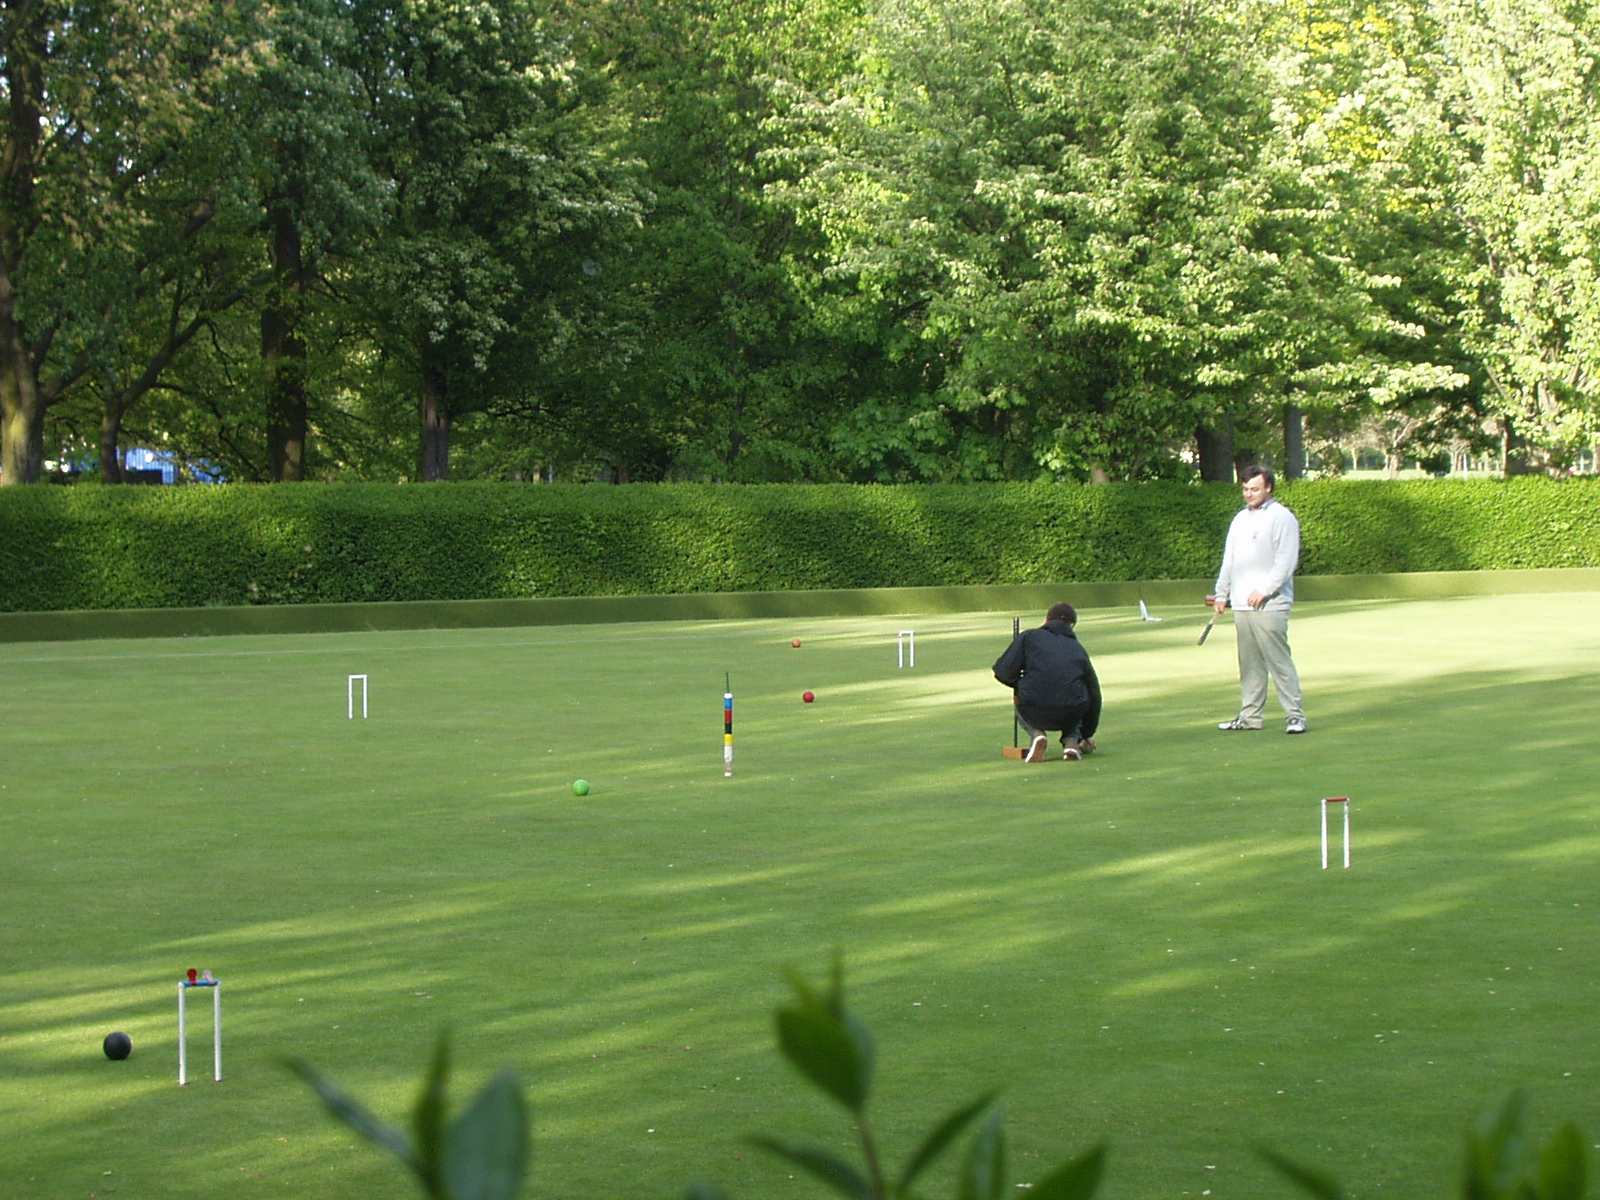
\includegraphics[width=0.8\linewidth]{images/krocketspieler.jpg}
    \caption{Krocketspieler in Edinburgh, Schottland. User:pschemp, CC BY-SA 3.0 <http://creativecommons.org/licenses/by-sa/3.0/>, via Wikimedia Commons}

\end{figure}

Es wird zunächst die Aufgabe beschrieben:

\textbf{Aufgabentext aus der 1. Runde des 43. Bundeswettbewerbs Informatik:}
\begin{quote}
	``Laura findet beim Spielen im Garten einige aufgestellte Tore eines Krocketspiels. Ihr Vater ruft aus der Küche, dass er es mit nur zwei Schlägen geschafft hat, den Ball durch alle Tore in der richtigen Reihenfolge zu stoßen. Das möchte Laura verbessern, wobei sie sich allerdings erlaubt, von einem selbst gewählten Punkt aus abzuschlagen. Aber geht das überhaupt?
	
	Aufgabe 4: Hilf Laura, indem du ein Programm schreibst, das überprüft, ob alle Tore in der richtigen Reihenfolge mit nur einem Schlag durchquert werden können. Falls ja, soll dein Programm ein entsprechendes Paar aus Startpunkt und Schlagrichtung ausgeben. Der Ball ist rund und hat einen in der Eingabe angegebenen Radius $r$. Die Tore sehen von oben wie verschieden lange Geradensegmente aus und sind in der vorgeschriebenen Reihenfolge jeweils durch ihre zwei Endpunkte dargestellt. Hinweis: Es ist hilfreich, den Radius des Balls in einem ersten Lösungsversuch zu vernachlässigen, das heißt $r=0$ anzunehmen.'' \cite{aufgaben}
\end{quote}

Die Lösung der Aufgabe muss also überprüfen, ob es möglich ist, einen Ball mit nur einem einzigen Schlag so zu schießen, dass er alle Tore passiert. Dabei müssen sowohl der Ballradius $r$ als auch die Reihenfolge der Tore beachtet werden. Wenn der Ball alle Tore zwar durchschießen kann, aber nur in der falschen Reihenfolge, ist die Aufgabe nicht lösbar. Die Positionen und Anzahl der Tore sowie der Ballradius sind gegeben. Die Lösung muss eine Gerade $g_1$ zurückgeben. Diese Gerade muss einen Mindestabstand $r$ zu allen Toren haben, damit der Ball auf der Geraden durch alle Tore geschossen werden kann.

\subsection{Lösungsunabhängige Beobachtungen} 
\label{sec:beobachtungen}

Um die Aufgabe zu lösen und einen schnellen Algorithmus zu implementieren wird sich hier zunächst mit einigen wichtigen Beobachtungen auseinandergesetzt, welche essentiell sind um den folgenden Algorithmus zu verstehen.

Ein Tor besteht immer aus einer geraden Strecke. Diese Punkte entsprechen den Pfosten des Tors. Beim Durchschießen eines Tors liegt stets einer der Pfosten links vom Schusspfad und der andere rechts davon, welcher Pfosten links und welcher rechts ist, hängt von der Richtung ab mit der durch das Tor geschossen wird. Diese Konfiguration der linken und rechten Pfosten – die sogenannte \emph{lr-Konfiguration} – gibt also die Schussrichtung des Tors an und umgekehrt.

Bei jeder Aufgabe ist es das Ziel, vom ersten zum letzten Tor zu schießen. Das erste Tor wird im Folgenden als \(t_0\) und das letzte als \(t_n\) bezeichnet. Die Linie, die den linken Pfosten von \(t_0\) mit dem linken Pfosten von \(t_n\) verbindet, wird als \(ll\) benannt, da beide linke Pfosten miteinander verbunden sind. Analog entsteht durch die Verbindung der rechten Pfosten von \(t_0\) und \(t_n\) die Linie \(rr\). Die Tore \(t_0\) und \(t_n\) bilden zusammen mit den Linien \(ll\) und \(rr\) ein Viereck – das \emph{initiale Viereck} (\hyperref[fig:Initialviereck]{Abb. 2}).

\begin{figure}[h]
\label{fig:Initialviereck}
\centering
\begin{tikzpicture}[scale=1.9]

	\coordinate (t0L) at (0,2);   
	\coordinate (t0R) at (1,-1);  
	\coordinate (tnL) at (6,2.5);  
	\coordinate (tnR) at (7.5,0.5);  
	

	\fill[gray!10] (t0L) -- (t0R) -- (tnR) -- (tnL) -- cycle;
	
	\draw[thick] (t0L) -- (t0R) node[left, midway] {\(t0\)};
	\draw[thick] (tnL) -- (tnR) node[right, midway] {\(tn\)};
	
	\draw[dashed, blue, very thick] (t0L) -- (tnL) node[above, midway] {\(ll\)};
	\draw[dashed, red, very thick] (t0R) -- (tnR) node[below, midway] {\(rr\)};
	
\end{tikzpicture}
\caption{Initialviereck bestehend aus dem ersten Tor \(t_0\) und dem letzten Tor \(t_n\). Die linken und rechten Pfosten sind jeweils mit einer Linie \(ll\) bzw. \(rr\) verbunden. Jede mögliche Lösung muss durch dieses Initialviereck laufen.}

\end{figure}


Das Initialviereck, bestehend aus \(t_0\), \(t_n\), \(ll\) und \(rr\), stellt einen Kanal dar, durch den jeder mögliche Schuss verlaufen muss. Ist die lr-Konfiguration für jedes Tor bekannt, lässt sich ein \emph{Kanalpolygon} (\hyperref[fig:kanalpolygon]{Abb. 3a und 3b}) konstruieren, indem alle linken und rechten Pfosten in der richtigen Reihenfolge miteinander verbunden werden. Wenn sich die Verbindungsstrecken des Kanalpolygons überkreuzen, so ist die Aufgabe nicht lösbar, da die Tore entweder in der falschen Reihenfolge angeordnet sind oder kein Pfad durch das Kanalpolygon mehr führt. Daher muss zunächst überprüft werden, ob ein valides Kanalpolygon existiert.




\begin{figure}[t]
    \centering

    \vspace{-1cm} 
    \begin{subfigure}{\linewidth}
        \centering
        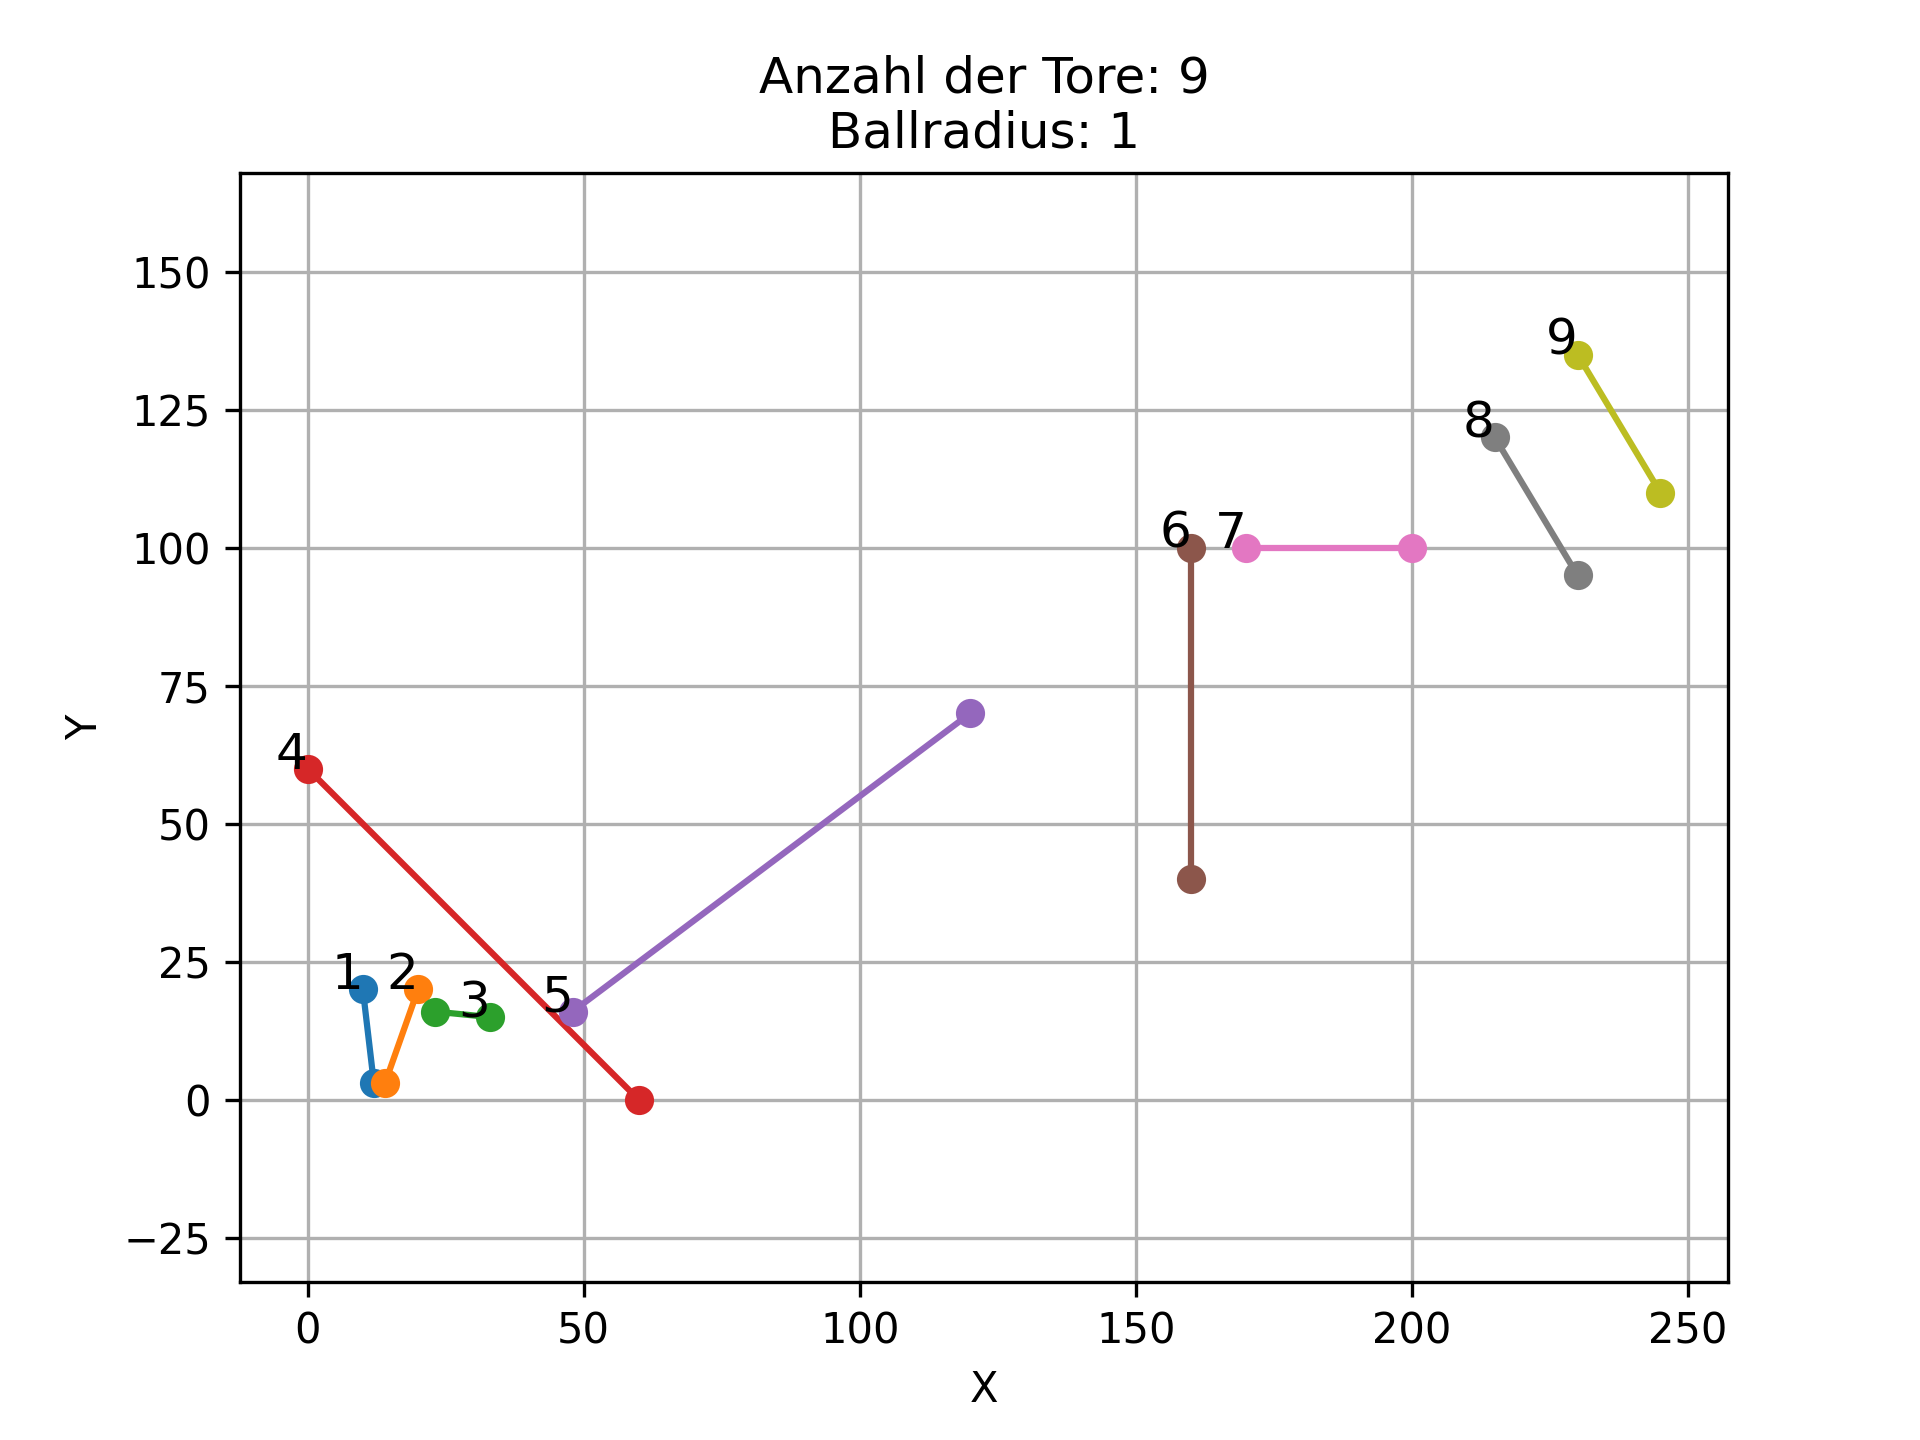
\includegraphics[width=0.8\linewidth]{images/krocket1.png}
        \caption{}
        \label{fig:tore}
    \end{subfigure}
    \vspace{-0.5cm}        

    \begin{subfigure}{\linewidth}
        \centering
        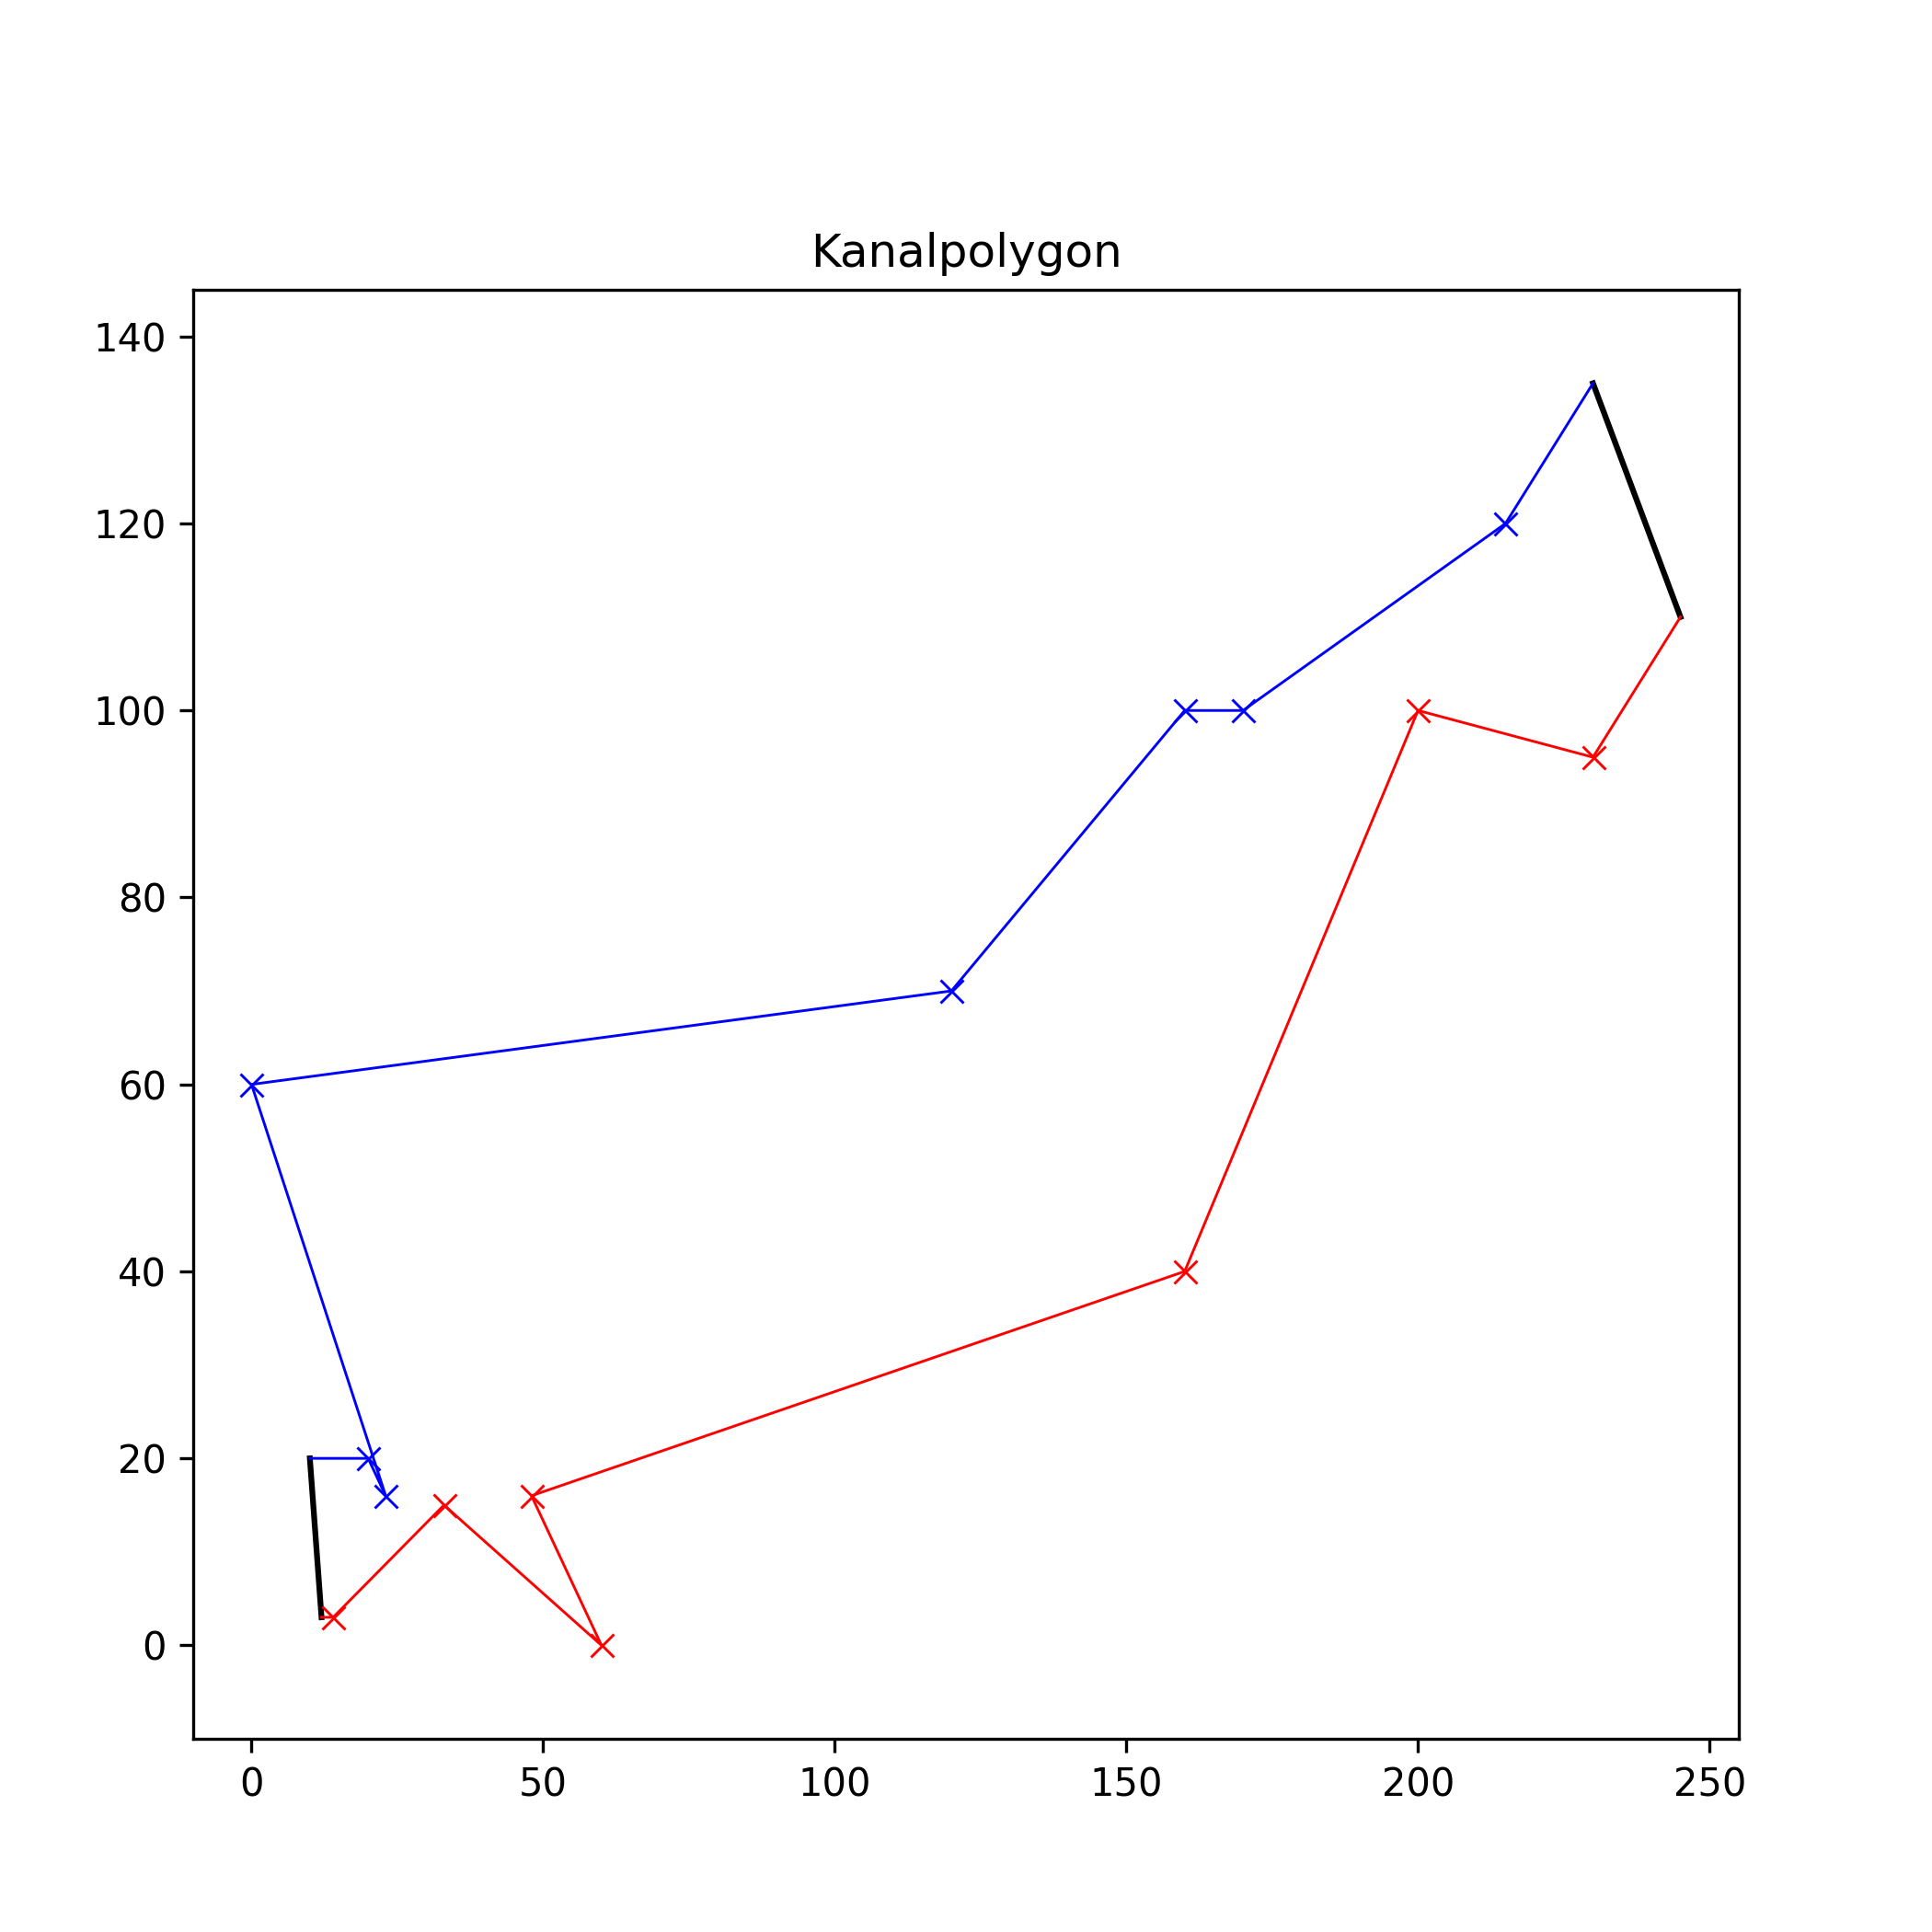
\includegraphics[width=0.8\linewidth]{images/testplot.png}
        \caption{}
        \label{fig:kanalpolygon}
    \end{subfigure}

    \caption{Vergleich zwischen Beispielaufgabe und Kanalpolygon. In Grafik (a) ist die Beispielaufgabe 1 aus dem 43. Bundeswettbewerb Informatik abgebildet. Alle Tore sind nummeriert und in unterschiedlichen Farben dargestellt. Aus dieser Aufgabe wird das Kanalpolygon in Grafik (b) erstellt, indem alle linken Pfosten (blau) und alle rechten Pfosten (rot) miteinander verbunden werden. Das erste Tor \(t_0\) und das letzte Tor \(t_n\) sind als schwarze Linien dargestellt.}
\end{figure}


\subsection{Aufbau des Algorithmus}
Für das Lösen der Aufgabe ist eine Aufteilung des Algorithmus sinnvoll. 
Der Algorithmus wird in zwei Teile geteilt:
\begin{enumerate}
    \item Im ersten Schritt überprüft der Algorithmus die Reihenfolge der Tore, um zu beurteilen, ob ein Durchschuss in der richtigen Reihenfolge überhaupt theoretisch möglich ist. Außerdem die lr-Konfiguration aller Tore gefunden werden, um so später ein Kanalpolygon erstellen zu können. Um diesen Punkt geht es in den Kapiteln \ref{sec:winkeltest} bis \ref{sec:ende_punkt_1}.

    \item Im zweiten Schritt werden sogenannte Chokepoints gefunden. Das sind Punkte, die das Kanalpolygon besonders stark einschränken. Dabei werden viele, für die Lösung nicht relevante Pfosten, herausgefiltert. Diese Pfosten haben Eigenschaften, welche spätere Verfahren unmöglich machen würden. Außerdem sind spätere Berechnungen deutlich komplizierter und eine geringere Anzahl an Pfosten beschleunigt den Algorithmus. Punkt 2 behandeln die Kapitel \ref{sec:anfang_2} bis \ref{sec:ende_2}.

    \item Im dritten Schritt muss der Algorithmus nach einer Geraden $g_1$ suchen, die durch alle Tore führt und einen Mindestabstand von dem Ballradius $r$ zu jedem Pfosten hat. In den Kapiteln \ref{sec:anfang_3} bis \ref{sec:ende_3} geht es um Punkt 3.


\end{enumerate}


Der Algorithmus für das Lösen der Aufgabe 4 des 43. Bundeswettbewerbs Informatik hat eine lineare Laufzeitkomplexität.
Ein Algorithmus mit linearer Laufzeitkomplexität ist ein Algorithmus, dessen Laufzeit in direktem Verhältnis zur Größe der Eingabe steht, seine Laufzeit also in etwa proportional zu \(n\) wächst. Das bedeutet, dass wenn sich die Anzahl der zu verarbeitenden Elemente verdoppelt, sich auch der Rechenaufwand verdoppelt und damit auch die Ausführungszeit verdoppelt. Ein Beispiel ist das sequentielle Durchlaufen einer Liste, bei dem jedes Element genau einmal bearbeitet wird. Ein linearer Algorithmus wird als O(n) klassifiziert. \cite{Cormen2009}



\subsection{Winkeltest}
\label{sec:winkeltest}

Der Winkeltest ist ein Tool, um die Reihenfolge von Toren zu überprüfen. Um dies zu testen werden alle Tore in ihrer möglichen lr-Konfiguration benötigt (Input), weil die lr-Konfiguration eines Tors die Richtung angibt, durch die das Tor durchschossen werden muss (vgl. \ref{sec:beobachtungen}). Der Winkeltest verarbeitet diese lr-Konfiguration und liefert als Ergebnis, ob alle Tore in der richtigen Reihenfolge liegen.

\subsubsection{Winkelberechnung}
Um die Reihenfolge der Tore zu überprüfen, werden für jeden Pfosten zwei Winkel betrachtet und berechnet (\hyperref[fig:winkeltest]{Abb. 4}):
\begin{enumerate}
	\item \textbf{Winkel $\lambda$ am linken Pfosten:} Zuerst wird der Winkel zwischen der Verbindungslinie vom linken Pfosten des aktuellen Tors zum rechten Pfosten desselben Tors und der Verbindungslinie vom rechten Pfosten des aktuellen Tors zum linken Pfosten des folgenden Tors gemessen.
	\item \textbf{Winkel $\rho$ am rechten Pfosten:} Zuerst wird der Winkel zwischen der Verbindungslinie vom rechten Pfosten des aktuellen Tors zum linken Pfosten desselben Tors und der Verbindungslinie vom linken Pfosten des aktuellen Tors zum rechten Pfosten des folgenden Tors gemessen.
\end{enumerate}

\begin{figure}[h]
\centering
\label{fig:winkeltest}
		\begin{tikzpicture}[scale=2]

		\coordinate (A) at (0.5,1);
		\coordinate (B) at (1.5,0);

		\coordinate (C) at (5,2);
		\coordinate (D) at (5.2,0);
		

		\fill (A) circle (2pt) node[below left] {A};
		\fill (B) circle (2pt) node[below right] {B};
		\fill (C) circle (2pt) node[above left] {C};
		\fill (D) circle (2pt) node[above right] {D};
	
		\draw[thick]  (A) -- (B);
		\draw[thick] (C) -- (D);
		
		\draw[->, red, thick, dashed] (A) -- (C);
		\draw[->, red, thick, dashed] (B) -- (D);
		
\draw pic[draw, angle eccentricity=1.2, angle radius=1cm, ultra thick, blue] 
    {angle = B--A--C} node[thick, anchor=center, text=blue] at ($(A)!0.5!(C) + (-1.9,-0.65)$) {$\lambda$};

\draw pic[draw, angle eccentricity=1.2, angle radius=1cm, ultra thick, blue] 
    {angle = D--B--A} node[thick, anchor=center, text=blue] at ($(A)!0.5!(C) + (-1.2, -1.2)$) {$\rho$};


	\end{tikzpicture}
    \caption{Visualisierung der Winkelberechnung. Abgebildet sind zwei Tore (A,B) und (C,D). Der Winkeltest berechnet die Winkel $\lambda$ und $\rho$, um anschließend zu beurteilen, ob man durch beide Tore in der richtigen Reihenfolge schießen kann.}
\end{figure}
\newpage

\subsubsection{Fallunterscheidung}
Ausgehend von der Winkelberechnung ergeben sich drei Fälle, die im folgenden unterschieden werden:
\begin{description}
	\item[Fall 1:] Beide Winkel sind kleiner als \(180^\circ\). Beide Pfosten des nächsten Tors liegen weiter rechts als die Pfosten des aktuell betrachteten Tors. Das nächste Tor liegt in der richtigen Richtung.
	\item[Fall 2:] Beide Winkel sind größer als \(180^\circ\). Beide Pfosten des nächsten Tors liegen weiter links als die Pfosten des aktuell betrachteten Tors. Somit liegt das nächste Tor in der falschen Richtung, und ein Durchschuss aller Tore in der richtigen Reihenfolge ist unmöglich.
	\item[Fall 3:] Ein Winkel ist größer, der andere kleiner als \(180^\circ\). Ein Pfosten des nächsten Tors liegt weiter links, der andere weiter rechts als das aktuell betrachtete Tor. Hieraus kann ein korrekter Durchschuss noch nicht ausgeschlossen werden.
\end{description}

Um für alle möglichen Torpositionen eine korrekte Beurteilung zu ermöglichen, muss die generelle Ausrichtung der Tore berücksichtigt werden – denn die Tore können auch von rechts nach links verlaufen. Wird entweder Fall 1 oder Fall 2 erstmals festgestellt, wird diese Information gespeichert. Tritt später der jeweils andere Fall auf, so ändert sich die Ausrichtung der Tore, und ein korrekter Durchschuss ist nicht mehr möglich.


\subsection{Orientierungstest}
Damit der Winkeltest funktioniert muss die lr-Konfiguration von jedem Tor bekannt sein. Diese Aufgabe übernimmt der Orientierungstest. Als Input nimmt der Orientierungstest alle Tore. Es wird über jedes Tor iteriert und die richtige lr-Konfiguration gespeichert. Der Orientierungstest gibt die lr-Konfiguration aller Tore zurück.

\subsubsection{Der Algorithmus des Orientierungstests}
Das Ziel des Orientierungstests besteht darin, alle Pfosten eindeutig als linke oder rechte Pfosten zu klassifizieren und somit die Durchschussrichtung aller Tore festzulegen. Im folgenden wird der Orientierungstest anhand von zwei Toren erläutert, dem vorherigen Tor \(t_{prev}\) und dem neuen Tor \(t_{neu}\).

Für jeden Pfosten des vorherigen Tors werden alle möglichen Verbindungen zu den Pfosten des neuen Tors konstruiert. Dabei entstehen zwei Linienpaare, benannt nach den Pfosten:
\[
ll,\quad rr\quad\And\quad lr,\quad rl.
\]
Für beide Linienpaare wird überprüft, ob sich die Linien schneiden. Kreuzt sich ein Linienpaar, so ist in der jeweiligen lr-Konfiguration kein Durchschuss möglich. Es existiert jedoch stets mindestens ein Paar, das sich nicht überkreuzt – dieses Paar bestimmt die lr-Konfiguration für das neue Tor (\hyperref[fig:orientierungstest]{Abb. 5}).


\begin{figure}[h]
\centering
\label{fig:orientierungstest}
\begin{tikzpicture}[scale=2]

	\coordinate (prevR) at (0,0);
	\coordinate (prevL) at (0.5, 2.5); 
	

	\coordinate (newR) at (5, -0.5);   
	\coordinate (newL) at (5, 3);  

	\draw[thick] (prevL) -- (prevR);
	\node[above left] at (prevL) {\(t_{prev}^{l}\)};
	\node[below left] at (prevR) {\(t_{prev}^{r}\)};
	
	
	\draw[thick] (newL) -- (newR);
	\node[above right] at (newL) {\(t_{neu}^{l}\)};
	\node[below right] at (newR) {\(t_{neu}^{r}\)};

	\draw[blue, thick] (prevL) -- (newL) node[midway, above] {\(ll\)};
	\draw[blue, thick] (prevR) -- (newR) node[midway, below] {\(rr\)};

	\draw[red, dashed, thick] (prevL) -- (newR) node[midway, above right] {\(lr\)};
	\draw[red, dashed, thick] (prevR) -- (newL) node[midway, above left] {\(rl\)};
\end{tikzpicture}
\caption{Visualisierung des Orientierungstests. Es sind zwei Tore \(t_{prev}\) und \(t_{neu}\) zu sehen. Ihre Pfosten sind durch die Linien \(ll, rr, lr\) und \(rl\) verbunden. Das Linienpaar \(lr\), \(rl\) besitzt einen Schnittpunkt, diese lr-Konfiguration ist also für das neue Tor nicht möglich. Die Linien \(ll\), \(rr\) schneiden sich nicht untereinander, diese lr-Konfiguration ist also die richtige und kann gespeichert werden.}
\end{figure}


\subsubsection{Sonderfall Bifurkation}
\label{sec:ende_punkt_1}
In manchen Fällen des Orientierungstests kann es dazu kommen, dass sich die Linien beider Paare nicht schneiden, was zu einer \emph{Bifurkation} (\hyperref[fig:bifurkation]{Abb. 6}), also einer Gabelung des Kanalpolygons, führt. Eine Bifurkation impliziert, dass das betreffende Tor in beide Richtungen durchschossen werden kann. Um solche Fälle zu filtern, wird der Winkeltest mit dem Orientierungstest kombiniert. Zunächst wird die lr-Konfiguration von \(t_0\) durch Testen beider Möglichkeiten initialisiert. Anschließend iteriert der Orientierungstest über jedes neue Tor und ermittelt alle möglichen lr-Konfigurationen zwischen benachbarten Toren. Der anschließende Winkeltest stellt sicher, dass die gewählte Konfiguration in dieselbe Schussrichtung wie die vorangegangenen Tore führt (mindestens ein Winkel muss kleiner als \(180^\circ\) sein). So wird in den folgenden Toren die richtige lr-Konfiguration für das Tor mit der Bifurkation gespeichert, da eine der beiden Schussrichtungen mit den folgenden Toren ausgeschlossen werden kann.

\begin{figure}[h]
\centering
\label{fig:bifurkation}
	\begin{tikzpicture}[scale=2]

		\coordinate (prevR) at (0,0);   
		\coordinate (prevL) at (0,4);    

		\coordinate (newL) at (2,2);   
		\coordinate (newR) at (4,2); 
		
		\draw[very thick] (prevL) -- (prevR);
		\node[above left] at (prevL) {\(t_{prev}^{l}\)};
		\node[below left] at (prevR) {\(t_{prev}^{r}\)};

		\draw[very thick] (newL) -- (newR);
		\node[above right] at (newL) {\(t_{neu}^{l/r}\)};
		\node[above right] at (newR) {\(t_{neu}^{l/r}\)};
		
		\draw[blue, thick] (prevL) -- (newL) node[midway, left] {\(ll\)};
		\draw[blue, thick] (prevR) -- (newR) node[midway, right] {\(rr\)};

		\draw[red, dashed, thick] (prevL) -- (newR) node[midway, above left] {\(lr\)};
		\draw[red, dashed, thick] (prevR) -- (newL) node[midway, above right] {\(rl\)};

	\end{tikzpicture}
    
    \caption{Orientierungstest im Fall einer Bifurkation. Es sind zwei Tore \(t_{prev}\) und \(t_{neu}\) abgebildet. Ihre Pfosten sind durch die Linien \(ll, rr, lr\) und \(rl\) verbunden. Beide Linienpaare (\(ll,\,rr\) und \(lr,\,rl\)) schneiden sich nicht, sodass das neue Tor in beide Richtungen durchschossen werden kann.}
\end{figure}


Mit der Kombination des Winkeltests und des Orientierungstests ist der erste Teil des Algorithmus abgeschlossen. Es ist möglich, die richtige Reihenfolge der Tore zu überprüfen und alle Pfosten in linke und rechte Pfosten einzuteilen. In dem nächsten Kapitel wird erklärt, wie unwichtige Pfosten gelöscht und besonders wichtige Pfosten gefunden werden.

\subsection{Chokepoints}
\label{sec:anfang_2}
Die Pfosten können jetzt mit Hilfe des Winkel- und Orientierungstest in rechte und linke Pfosten eingeteilt werden. Somit kann zwar ein Kanalpolygon erstellt werden, das allein reicht aber nicht für die Lösung. Das Kanalpolygon wird von allen Pfosten unterschiedlich stark eingegrenzt. Dabei existieren einzelne Pfosten, die das Kanalpolygon besonders stark einschränken. Diese kritischen Pfosten werden als \emph{Chokepoints} bezeichnet. Sie sind für das Berechnen der Schussgerade unabdingbar.\\

Die folgenden Abbildungen (\hyperref[fig:choke_equal]{Abb. 7} und \hyperref[fig:choke_diff]{Abb. 8}) verdeutlichen, dass die herkömmliche x- und y-Achsen-Aufteilung nicht ausreicht, um Chokepoints eindeutig zu bestimmen – es bedarf eines normierten Koordinatensystems (z.~B. basierend auf Isoklinen), um die relevanten Anteile der Höhe zwischen \(t_0\) und \(t_n\) zu erfassen.

\begin{figure}[h]
\centering
\label{fig:choke_equal}
    \begin{tikzpicture}[scale=2]

        \coordinate (t0R) at (0,0);
        \coordinate (t0L) at (0.5, 4);
        \coordinate (tnR) at (4.5, 0);
        \coordinate (tnL) at (4,4);

        \draw[thick] (t0L) -- (t0R);
        \draw[thick] (tnL) -- (tnR);
        \node[above left] at (t0L) {\(t_0^{l}\)};
        \node[below left] at (t0R) {\(t_0^{r}\)};
        \node[above right] at (tnL) {\(t_n^{l}\)};
        \node[below right] at (tnR) {\(t_n^{r}\)};

        \draw[gray, fill=gray!20] (t0L) -- (t0R) -- (tnR) -- (tnL) -- cycle;

        \coordinate (Cleft) at (2, 1.5);

        \coordinate (Cright) at (3,1.5);

        \draw[ultra thick, red] (t0R) -- (Cleft) -- (Cright) -- (tnR);
        \filldraw[red] (Cleft) circle (2pt) node[above left] {\(C_1\)};
        \filldraw[red] (Cright) circle (2pt) node[above right] {\(C_2\)};
        
    \end{tikzpicture}
    
	\caption{Chokepoints mit gleichem Einfluss auf das Kanalpolygon. Darstellung von zwei Chokepoints mit gleichem y-Wert \(C_1\) und \(C_2\), außerdem sind zwei Tore \(t_0\) und \(t_n\) abgebildet. Die schwarzen Linien sind das Initialpolygon und die roten Linien sind das Kanalpolygon. Beide Chokepoints schränken das Kanalpolygon ungefähr gleich stark ein.}
\end{figure}

\vspace{5cm}

\begin{figure}[h]
\centering
\label{fig:choke_diff}
	\begin{tikzpicture}[scale=2]

	\coordinate (t0R) at (0,0);
	\coordinate (t0L) at (0, 2);
	\coordinate (tnR) at (4, 0);
	\coordinate (tnL) at (4,6);
	
	\draw[thick] (t0L) -- (t0R);
	\draw[thick] (tnL) -- (tnR);
	\node[below left] at (t0L) {\(t_0^{l}\)};
	\node[below right] at (t0R) {\(t_0^{r}\)};
	\node[above left] at (tnL) {\(t_n^{l}\)};
	\node[above right] at (tnR) {\(t_n^{r}\)};
	
	\draw[gray, fill=gray!20] (t0L) -- (t0R) -- (tnR) -- (tnL) -- cycle;
	

	\coordinate (Cleft) at (0.75, 1.5);

	\coordinate (Cright) at (3,1.5);
	
	\draw[ultra thick, red] (t0R) -- (Cleft) -- (Cright) -- (tnR);
	\filldraw[red] (Cleft) circle (2pt) node[above left] {\(C_1\)};
	\filldraw[red] (Cright) circle (2pt) node[above right] {\(C_2\)};

	\end{tikzpicture}

    \caption{Chokepoints mit unterschiedlichem Einfluss auf das Kanalpolygon. Darstellung von zwei Chokepoints mit gleichem y-Wert \(C_1\) und \(C_2\), außerdem sind zwei Tore \(t_0\) und \(t_n\) abgebildet, \(t_0\) ist wesentlich kleiner als \(t_n\). Die schwarzen Linien stellen das Initialpolygon und die roten Linien  das Kanalpolygon dar. \(C_1\) schränkt das Kanalpolygon deutlich stärker ein als \(C_2\), obwohl beide im Koordinatensystem auf gleicher y-Höhe liegen.}
\end{figure}

\vspace{1em}

Aus den Beispielen lässt sich ableiten, dass die klassischen x- und y-Werte nicht sinnvoll zur Ermittlung von Chokepoints sind. Auch die Betrachtung von \(t_0\) und \(t_n\) als y-Achse bzw. \(ll\) und \(rr\) als x-Achse erweist sich als unzureichend, da diese Linien weder parallel zur x-/y-Achse noch untereinander parallel verlaufen müssen.

\newpage
\subsubsection{Verzerrte Ebene und Isoklinen}
\label{sec:ebene}
Um die im letzten Kapitel beschriebene Problematik zu überwinden, wird eine verzerrte Ebene eingeführt. Innerhalb eines beliebigen Vierecks kann so ein normiertes Koordinatensystem konstruiert werden, das die Pfosten relativ zueinander vermisst. Hierbei kommen Linien mit gleichen Abstandsproportionen zum Einsatz, die als \emph{Isoklinen} bezeichnet werden. Analog zu geographischen Koordinaten werden \emph{Längengrad-Isoklinen} (vergleichbar mit der x-Achse) und \emph{Breitengrad-Isoklinen} (vergleichbar mit der y-Achse) aufgebaut. Jeder Pfosten im initialen Viereck wird einer Steigung in Richtung des größeren Tores bzw. der längeren Linie (\(ll\) oder \(rr\)) zugeordnet.

Die Längengrad-Isoklinen geben an, wie nahe ein Pfosten an \(t_n\) liegt: Ein Pfosten auf \(t_0\) besitzt den Längengrad 0, während ein Pfosten auf \(t_n\) den Längengrad 1 aufweist. Die Breitengrad-Isoklinen bestimmen, wie nah ein Pfosten an \(rr\) liegt: Ein Breitengrad von 0 bedeutet, dass der Pfosten auf \(ll\) liegt, während ein Breitengrad von 1 anzeigt, dass der Pfosten auf \(rr\) liegt. So besitzt beispielsweise der linke Pfosten von \(t_0\) im normierten Koordinatensystem die Koordinaten \((0,0)\). Dies ermöglicht die Betrachtung des Problems im Einheitsquadrat – jeder Punkt ist eindeutig zuzuordnen. Ein Punkt, der 50\% des Wegs von \(t_0\) zu \(t_n\) zurückgelegt hat, liegt beispielsweise auf der 0,5-Längengrad-Isokline.

\subsubsection{Konstruktion von Längen- und Breitengrad-Isoklinen}
Für jeden Pfosten müssen die Längen- und Breitengrad-Isoklinen berechnet werden (\hyperref[fig:isoklinen]{Abb. 9}). Sind beispielsweise die Linien \(t_0\) und \(t_n\) parallel, verlaufen die Längengrad-Isoklinen ebenfalls parallel zu diesen Linien. In den meisten Fällen sind die Linienpaare jedoch nicht parallel, sodass deren charakteristische Funktionen einen gemeinsamen Schnittpunkt – den \emph{Ursprung} – besitzen. Dieser liegt außerhalb des Kanalpolygons. Für jeden Pfosten wird eine Isokline konstruiert, die den Pfosten mit diesem Urspung verbindet. Der Punkt, an dem die Isokline die kleinere der beiden Linien schneidet, dient zur Berechnung des relativen Abstands (Breite bzw. Länge) des Pfostens. Über diesen Ansatz können auch die Chokepoints identifiziert werden, die dem globalen Maximum der Breitengrad-Isoklinen entsprechen (sowohl für alle linken als auch für alle rechten Pfosten).


\begin{figure}[H]
\centering
\label{fig:isoklinen}
\begin{tikzpicture}[scale=1.5]

    \coordinate (A) at (1,1);
    \coordinate (B) at (0,3);
    \coordinate (C) at (4.5,5);
    \coordinate (D) at (3.5,-0.5);
    
    \draw[fill=gray!20, draw=black] (A) -- (B) -- (C) -- (D) -- cycle;
    
    \draw[thick, name path=t0] (A) -- (B) node[midway, left] {\(t_0\)};
    \draw[thick, name path=tn] (D) -- (C) node[midway, right] {\(t_n\)};
    
    \draw[blue, very thick, name path=ll] (A) -- (D) node[midway, below] {\(rr\)};
    \draw[blue, very thick, name path=rr] (B) -- (C) node[midway, above] {\(ll\)};
    
    \draw[dashed, gray] (A) -- ($ (B)!4!(A) $);
    \draw[dashed, gray] (D) -- ($ (C)!2!(D) $);
    \draw[dashed, gray] (A) -- ($ (D)!3!(A) $);
    \draw[dashed, gray] (B) -- ($ (C)!2!(B) $);
    
    \coordinate (A2) at (3.0333,-3.0667);
    \filldraw[red] (A2) circle (2pt) node[right] {\(U_2\)};
    
    \coordinate (A1) at (-1.34,2.41);
    \filldraw[green!70!black] (A1) circle (2pt) node[above] {\(U_1\)};
    

    \coordinate (P) at (2,2);
    \filldraw[black] (P) circle (2pt) node[above right] {\(P\)};
    
    \path[name path=Liso] (P) -- (A2);
    \draw[dashed, red] (P) -- (A2);
    
    \coordinate (S1) at (0.4,2.19);
    \filldraw[green!70!black] (S1) circle (2pt) node[above right] {\(S_1\)};
    \draw[dotted, green!70!black] (P) -- (S1);
    
    \path[name path=Biso] (P) -- (A1);
    \draw[dashed, green!70!black] (P) -- (A1);
    
    \coordinate (S2) at (2.35,0.2);
    \filldraw[red] (S2) circle (2pt) node[above right] {\(S_2\)};
    \draw[dotted, red] (P) -- (S2);
    
\end{tikzpicture}
\caption{Konstruktion von Längen- und Breitengrad-Isoklinen. Dargestellt sind zwei Linienpaare: die Tore \(t_0\), \(t_n\) und die Linien \(ll\) und \(rr\). Dort wo sich die erweiterten Linienpaare kreuzen, liegen die Urspünge \(U_1\) und \(U_2\). Von beiden Ursprüngen wird eine Linie, die jeweilige Isokline, zu dem Pfosten \(P\) gezogen. Die Schnittpunkte \(S_1\) und \(S_2\) der Isoklinen mit \(t_0\) bzw. \(rr\) sind markiert. Um die Isoklinenwerte zu berechnen wird die Lage des Schnittpunktes auf der jeweiligen Linie gemessen und als Wert zwischen 0 und 1 gespeichert.}
\end{figure}



\subsubsection{Filterung irrelevanter Pfosten}
\label{sec:ende_2}
Viele Pfosten im Kanalpolygon sind für die Bestimmung des gültigen Schusspfads irrelevant, da sie diesen nicht einschränken. Beim Berechnen der Isoklinen und bei der Suche nach Chokepoints können solche Pfosten herausgefiltert werden. Liegt der aktuelle Pfosten in Bezug auf den Längengrad niedriger als der vorherige, so befindet er sich näher an \(t_0\) – dies entspricht einer Bewegung „zurück“. Daraus entsteht ein Bereich im Kanalpolygon, der nicht Teil eines gültigen Schusspfads sein kann. Für das Herausfiltern solcher Bereiche sind die Steigungen der zwei letzten Streckensegmente des Kanalpolygons wichtig, einmal die Strecke von dem neuen Pfosten zu dem letzten (die neue Steigung) und die Strecke von dem letzten Pfosten zu dem vorletzten (die alte Steigung).

Um diese Situation zu differenzieren, werden folgende sechs Fälle betrachtet:
\begin{enumerate}
	\item Der neue Pfosten hat einen geringeren Breiten- und Längengrad als der vorherige Pfosten und die Steigungen haben unterschiedliche Vorzeichen.
	\begin{itemize}
		\item \textbf{Ergebnis:} Der vorherige Pfosten ist relevant, der neue ist irrelevant.
	\end{itemize}
	\item Der neue Pfosten hat einen geringeren Breiten- und Längengrad als der vorherige, die Steigungen haben gleiche Vorzeichen und die absolute neue Steigung ist größer als die absolute alte.
	\begin{itemize}
		\item \textbf{Ergebnis:} Der vorherige Pfosten ist relevant, der neue ist irrelevant.
	\end{itemize}
	\item Der neue Pfosten hat einen geringeren Breiten- und Längengrad als der vorherige, die Steigungen haben gleiche Vorzeichen und die absolute neue Steigung ist kleiner als die absolute alte.
	\begin{itemize}
		\item \textbf{Ergebnis:} Der vorherige Pfosten ist irrelevant, der neue ist relevant.
	\end{itemize}
	\item Der neue Pfosten hat einen geringeren Breitengrad, aber einen höheren Längengrad als der vorherige, und die Steigungen haben unterschiedliche Vorzeichen.
	\begin{itemize}
		\item \textbf{Ergebnis:} Der vorherige Pfosten ist irrelevant, der neue ist relevant.
	\end{itemize}
	\item Der neue Pfosten hat einen geringeren Breitengrad, aber einen höheren Längengrad als der vorherige, die Steigungen haben gleiche Vorzeichen und die absolute neue Steigung ist größer als die absolute alte.
	\begin{itemize}
		\item \textbf{Ergebnis:} Der vorherige Pfosten ist irrelevant, der neue ist relevant.
	\end{itemize}
	\item Der neue Pfosten hat einen geringeren Breitengrad, aber einen höheren Längengrad als der vorherige, die Steigungen haben gleiche Vorzeichen und die absolute neue Steigung ist kleiner als die absolute alte.
	\begin{itemize}
		\item \textbf{Ergebnis:} Der vorherige Pfosten ist relevant, der neue ist irrelevant.
	\end{itemize}
\end{enumerate}

So konnten bereits viele unwichtige Pfosten herausgefiltert werden. Übrig bleiben einzelne lokale Extremwerte (lokale Breitengrad-Minima), die entfernt werden können, um die Anzahl der Pfosten weiter zu reduzieren und so die Kanallinien zu glätten. Diese unwichtigen Pfosten muss der Algorithmus bei der Schusspfadberechnung nicht mehr beachten, wodurch der Algorithmus schneller wird. 


\subsection{Schusspfadberechnung}
\label{sec:anfang_3}
Im Folgenden wird die Schusspfadberechnung erläutert. Mithilfe der nicht aussortierten Pfosten sowie der Chokepoints wird der letzte Teil des Algorithmus erklärt, der die Lösung der Aufgabe berechnet und konstruiert. Ziel dieser Berechnung ist es, einen Schuss zu finden, der alle relevanten Tore in der vorgegebenen Reihenfolge passiert.

Um diesen Teil des Algorithmus zu ermöglichen, wurden im Vorfeld die Reihenfolge der Tore überprüft, die \textit{lr-Konfiguration} aller Tore gefunden, die Längen- und Breitengrad-Isoklinen der Tore berechnet, die Chokepoints gefunden und nicht relevante Pfosten herausgefiltert. Für das finden einer Lösung muss nach mehreren wichtigen Pfosten gesucht werden. Wie diese Pfosten charakterisiert und gefunden werden, wird im nächsten Unterkapitel erläutert.


\newpage
\subsubsection{Stützpfosten} 
Neben den Chokepoints spielt die Bestimmung zusätzlicher Stützpfosten eine entscheidende Rolle. Stützpfosten sind Pfosten, auf denen ein möglicher Schusspfad liegen kann, sie sind essentiell zum Finden einer Lösung. Dabei wird zwischen zwei Arten von Stützpfosten unterschieden.

\paragraph{Hauptstützpfosten:}
Für alle linken und alle alle rechten Pfosten wird separat der Winkel berechnet, der sich zwischen der Verbindungslinie von $t_n$ links/rechts zu $t_0$ links/rechts und der Verbindungslinie zu dem betreffenden Pfosten ergibt. Der Pfosten mit dem kleinsten Winkel wird als Hauptstützpfosten definiert (\hyperref[fig:hauptpfosten]{Abb. 10}). Er fungiert als eine Art „Anti Chokepoint“, da er als erster kritischer Pfosten in der Schussbahn wirkt, wenn in Richtung „links oben“ geschossen wird. 

\begin{figure}[h]
\centering
\label{fig:hauptpfosten}
 \begin{tikzpicture}[scale=2]

  \coordinate (t0R) at (0,0);
  \coordinate (tnR) at (4,0);
  \coordinate (t0L) at (1,4);
  \coordinate (tnL) at (5,4);

  \draw[thick] (t0L) -- (t0R);
  \draw[thick] (tnL) -- (tnR);
  \node[above left] at (t0L) {\(t_0^l\)};
  \node[above right] at (tnL) {\(t_n^l\)};
  \node[below left] at (t0R) {\(t_0^r\)};
  \node[below right] at (tnR) {\(t_n^r\)};

  \draw[dashed, blue] (t0L) -- (tnL) node[midway, above] {\(ll\)};
  \draw[dashed, blue] (t0R) -- (tnR) node[midway, below] {\(rr\)};

  \coordinate (P) at (3,2.1);
  \filldraw[green!70!black] (P) circle (2pt) node[above left] {\(P\)};

  \draw[thick, ->] (tnL) -- (P);

\draw pic[draw, green!70!black, very thick, angle radius=1.5cm, angle eccentricity=1.5, text={"$\theta_P$"}] {angle = P--tnL--t0L};
  \node[green!70!black, very thick] at (5.7, 4.7) {\(\theta_P\)};

  \coordinate (CP_left) at (1,1.5);

  \coordinate (CP_right) at (3.4,1.7);
 
  \draw[ultra thick, blue] (t0L) -- (CP_left) -- (tnL);
  \draw[ultra thick, red] (t0R) -- (CP_right) -- (tnR);

  \filldraw[blue] (CP_left) circle (2pt) node[above left] {\(C_l\)};
  \filldraw[red] (CP_right) circle (2pt) node[above right] {\(C_r\)};
  
\end{tikzpicture}
    \caption{Berechnung von Hauptstützpfosten. Die Abbildung zeigt das Initialpolygon bestehend aus \(t_0\), \(t_n\), \(ll\) und \(rr\). Das Kanalpolygon ist durch die Chokepoints \(C_l\) und \(C_r\) vereinfacht dargestellt. Die Berechnung des Winkels \(\theta_P\) ist an einem Pfosten \(P\) beispielhaft dargestellt. Der Winkel \(\theta\) wird im Uhrzeigersinn von der Linie \(ll\) zu der Verbindungslinie von \(t^l_n\) nach \(P\) gemessen. Wenn \(\theta_P\) der größte Winkel von den linken Pfosten ist, ist \(P\) der linke Hauptstützpfosten.}
\end{figure}

\newpage

\paragraph{Untergeordnete Stützpfosten:}
Es gibt zwei linke und und zwei rechte untergeordnete Stützpfosten, jeweils einen für den Hauptstützpfosten und einen für den Chokepoint.
Für die Berechnung der zwei untergeordneten Stützpfosten (\hyperref[fig:unterpfosten]{Abb. 11}) werden für die linken Pfosten zusätzlich die zwei Winkel von $t_n$ rechts über den Chokepoint und über den Hauptstützpfosten zu den verbleibenden Pfosten berechnet. Die Pfosten, bei denen einer dieser Winkel am größten ist, werden als untergeordnete Stützpfosten bestimmt. Analog werden diese Berechnungen auch bei den rechten Pfosten vorgenommen. Der Pfad ausgehend von dem linken Chokepoint zu seinem untergeordneten Stützpfosten ist der flachste Pfad an allen linken Pfosten vorbei ausgehend von diesem Chokepoint. Das gilt auch für den Hauptstützpfosten und seinen untergeordneten Stützpfosten.

\begin{figure}[H]
\centering
\label{fig:unterpfosten}
 \begin{tikzpicture}[scale=2.5]

  \coordinate (t0R) at (0,0);
  \coordinate (tnR) at (4,0);
  \coordinate (t0L) at (1,4);
  \coordinate (tnL) at (5,4);

  \coordinate (CP_left) at (1,1.5);

  \coordinate (CP_right) at (3.4,1.7);

  \draw[thick] (t0L) -- (t0R);
  \draw[thick] (tnL) -- (tnR);
  \node[above left] at (t0L) {\(t_0^l\)};
  \node[above right] at (tnL) {\(t_n^l\)};
  \node[below left] at (t0R) {\(t_0^r\)};
  \node[below right] at (tnR) {\(t_n^r\)};

  \draw[dashed, blue] (t0L) -- (tnL) node[midway, above] {\(ll\)};
  \draw[dashed, blue] (t0R) -- (tnR) node[midway, below] {\(rr\)};

\coordinate (P) at (2,1.5);

  \draw[thick] (CP_left) -- (P);
  \draw[thick] (tnR) -- (CP_left);

    \filldraw[green!70!black] (P) circle (2pt) node[above left] {\(P\)};

  \draw[ultra thick, blue] (t0L) -- (CP_left) -- (tnL);
  \draw[ultra thick, red] (t0R) -- (CP_right) -- (tnR);

  \filldraw[blue] (CP_left) circle (2pt) node[above left] {\(C_l\)};
  \filldraw[red] (CP_right) circle (2pt) node[above right] {\(C_r\)};
  
\draw pic[draw, green!70!black, very thick, angle radius=1.4cm, angle eccentricity=1.5, text={"$\theta_P$"}] {angle = P--CP_left--tnR};
  \node[green!70!black, very thick] at (0.6, 0.9) {\(\theta_P\)};
  
\end{tikzpicture}
    \caption{Berechnung von untergeordneten Stützpfosten. Die Abbildung zeigt das Initialpolygon bestehend aus \(t_0\), \(t_n\), \(ll\) und \(rr\). Das Kanalpolygon ist durch die Chokepoints \(C_l\) und \(C_r\) vereinfacht dargestellt. Die Berechnung des Winkels \(\theta_P\) ist an einem Pfosten \(P\) beispielhaft dargestellt. Der Winkel \(\theta\) wird im Uhrzeigersinn von der Linie von \(t^r_n\) nach \(C_l\) zu der Verbindungslinie von \(C_l\) nach \(P\) gemessen. Wenn \(\theta_P\) der größte Winkel von den linken Pfosten ist, ist \(P\) der linke untergeordnete Stützpfosten des linken Hauptstützpfosten.}
\end{figure}

\newpage
\subsubsection{Konfigurationen des Kanalpolygons} 
\label{sec:ende_3}
Liegt der Breitengrad des linken Chokepoints höher als der des rechten, also der linke Chokepoint weiter unten als der rechte, spricht man von einer Breiten Konfiguration. Diese spezielle Position der Chokepoints erfordert eine abweichende Behandlung im weiteren Verlauf der Konstruktion und Berechnung.

\paragraph{Breite Konfiguration:}

Bei einer breiten Konfiguration kann eine einfache Probe durchgeführt werden, indem die Isoklinen der beiden Chokepoints getestet werden, um zu überprüfen, ob diese bereits zu einem gültigen Schusspfad führen.
Wenn dies nicht der Fall ist sind für linke und für rechte Pfosten folgende beiden Pfostenpaare interessant: der Chokepoint und dessen untergeordneter Stützpfosten, sowie der Hauptstützpfosten und dessen untergeordneter Stützpfosten.

Für jedes mögliche Paar dieser Pfosten wird eine mögliche Lösung konstruiert, indem entweder eine lineare Funktion bestimmt wird, die durch beide Pfosten verläuft oder zwei Pfosten aus gegenüberliegenden Kanälen zu einer möglichen Lösung verbunden werden. Die Strecke zwischen den beiden Pfosten stellt damit die Diagonale eines Segments des Schusskanals dar. Somit kann diese Diagonale als Hypothenuse eines rechtwinkligen Dreiecks dazu verwendet werden, um den Rest des Schusspfads zu konstruieren. Dabei ist die Höhe des Kanals jeweils die Ankathete der Pfosten, die zur Konstruktion herangezogen wurden. Es werden für alle acht Pfosten alle möglichen Paare überprüft. Danach wird der Abstand von dieser Funktion zu jedem Pfosten auf der anderen Seite (bei einer Funktion aus linken Pfosten also für jeden rechten Pfosten) gemessen, wobei der kleinste Abstand gespeichert wird. Als letztes wird eine Parallele von der linearen Funktion mit diesem kleinsten Abstand konstruiert und überprüft, ob diese beiden parallelen Linien einen Schnittpunkt mit allen anderen Toren aufweisen (\hyperref[fig:schusspfad]{Abb. 12}). Wenn dies der Fall ist, wurde eine gültige Lösung gefunden. Wird für kein Pfostenpaar eine Lösung gefunden, gibt es für die Aufgabe keine Lösung.

\paragraph{Keine breite Konfiguration:}
Wenn keine breite Konfiguration vorliegt, der linke Chokepoint also einen höheren Längengrad als der rechte hat, müssen die Isoklinen nicht als mögliche Lösungen ausprobiert werden, da diese nicht funktionieren können. Es kann also sofort mit der Überprüfung der Pfostenpaare gestartet werden. Danach verläuft alles analog zur breiten Konfiguration, es werden also die Parallelen aus jedem Pfostenpaar konstruiert und anschließend wird überprüft, ob sie einen Schnittpunkt mit jedem Tor besitzen.

\begin{figure}[h]
\centering
\label{fig:schusspfad}
\begin{tikzpicture}[scale=1]

  \draw[thick] (0.5,1) -- (0.6,0.15) node[midway, left] {G1};

  \draw[thick] (1,1) -- (0.7,0.15) node[midway, below right] {G2};

  \draw[thick] (1.65,0.75) -- (1.15,0.8) node[midway, above] {G3};

  \draw[thick] (0,3) -- (3,0) node[midway, above right] {G4};

  \draw[thick] (2.4,0.8) -- (6,3.5) node[midway, above left] {G5};

  \draw[thick] (8,5) -- (8,2) node[midway, right] {G6};

  \draw[thick] (8.5,5) -- (10,5) node[midway, above] {G7};

  \draw[thick] (10.75,6) -- (11.5,4.75) node[midway, below right] {G8};

  \draw[thick] (11.5,6.75) -- (12.25,5.5) node[midway, below right] {G9};
  

\draw[thick, blue] (0,-0.05) -- (13,6.8) node[above right] {\(P_1\)};
\draw[thick, blue] (0,0.05) -- (13,6.9) node[below right] {\(P_2\)};
 
\end{tikzpicture}
\caption{Lösungsüberprüfung von zwei Parallelen.
Die Abbildung zeigt neun Torsegmente (\(G1\) bis \(G9\)). Außerdem sind zwei Parallelen \(P_1\) und \(P_2\) zu sehen. Sie stellen den Schusspfad des Balls dar. Da beide Parallelen einen Schnittpunkt mit jedem Tor besitzen ist dieser Schusspfad eine gültige Lösung.}
\end{figure}

Diese Schusspfadkonstruktion stellt damit den abschließenden Baustein des linearen Lösungsansatzes dar und ergänzt die zuvor beschriebenen Schritte zur Überprüfung der Tore sowie zur Filterung unwichtiger Pfosten. Dieser Algorithmus ermöglicht eine effiziente Lösung der Aufgabe 4 des 43. Bundeswettbewerbs Informatik.


\subsection{Umsetzung}

Neben den o.g. Betrachtungen zur theoretischen Erarbeitung des linearen Algorithmus ist ein weiterer Bestandteil meiner Komplexen Leistung die praktische Umsetzung. Aufgrund des limitierten Umfangs der Komplexen Leistung kann ich nur sehr kurz auf die Implementierung des Algorithmus eingehen.
Der Code ist ausschließlich in Python geschrieben. Er ist öffentlich auf Github zugänglich und dort auch ausführlich dokumentiert \cite{implementierung}. 

Sowohl die theoretische Erarbeitung des Algorithmus, als auch die Implementierung des Algorithmus habe ich zusammen mit Max Polter erarbeitet. Dabei habe ich den gesamten Code des Winkel- und Orientierungstest geschrieben, sowie Teile des Kanalpolygons und der Chokepointsuche. Den Algorithmus haben wir in großen Teilen zusammen erarbeitet. Er kann alle Beispielaufgaben des 43. Bundeswettbewerb Informatik lösen \cite{beispielaufgaben}. In den folgenden Abbildungen (\hyperref[fig:beispiele]{Abb. 13}) und (\hyperref[fig:beispiele2]{Abb. 14}) werden die Ergebnisse des Algorithmus dargestellt.

\begin{figure}[h]
\label{fig:beispiele}
     \centering
     \begin{subfigure}[b]{0.49\textwidth}
         \centering
         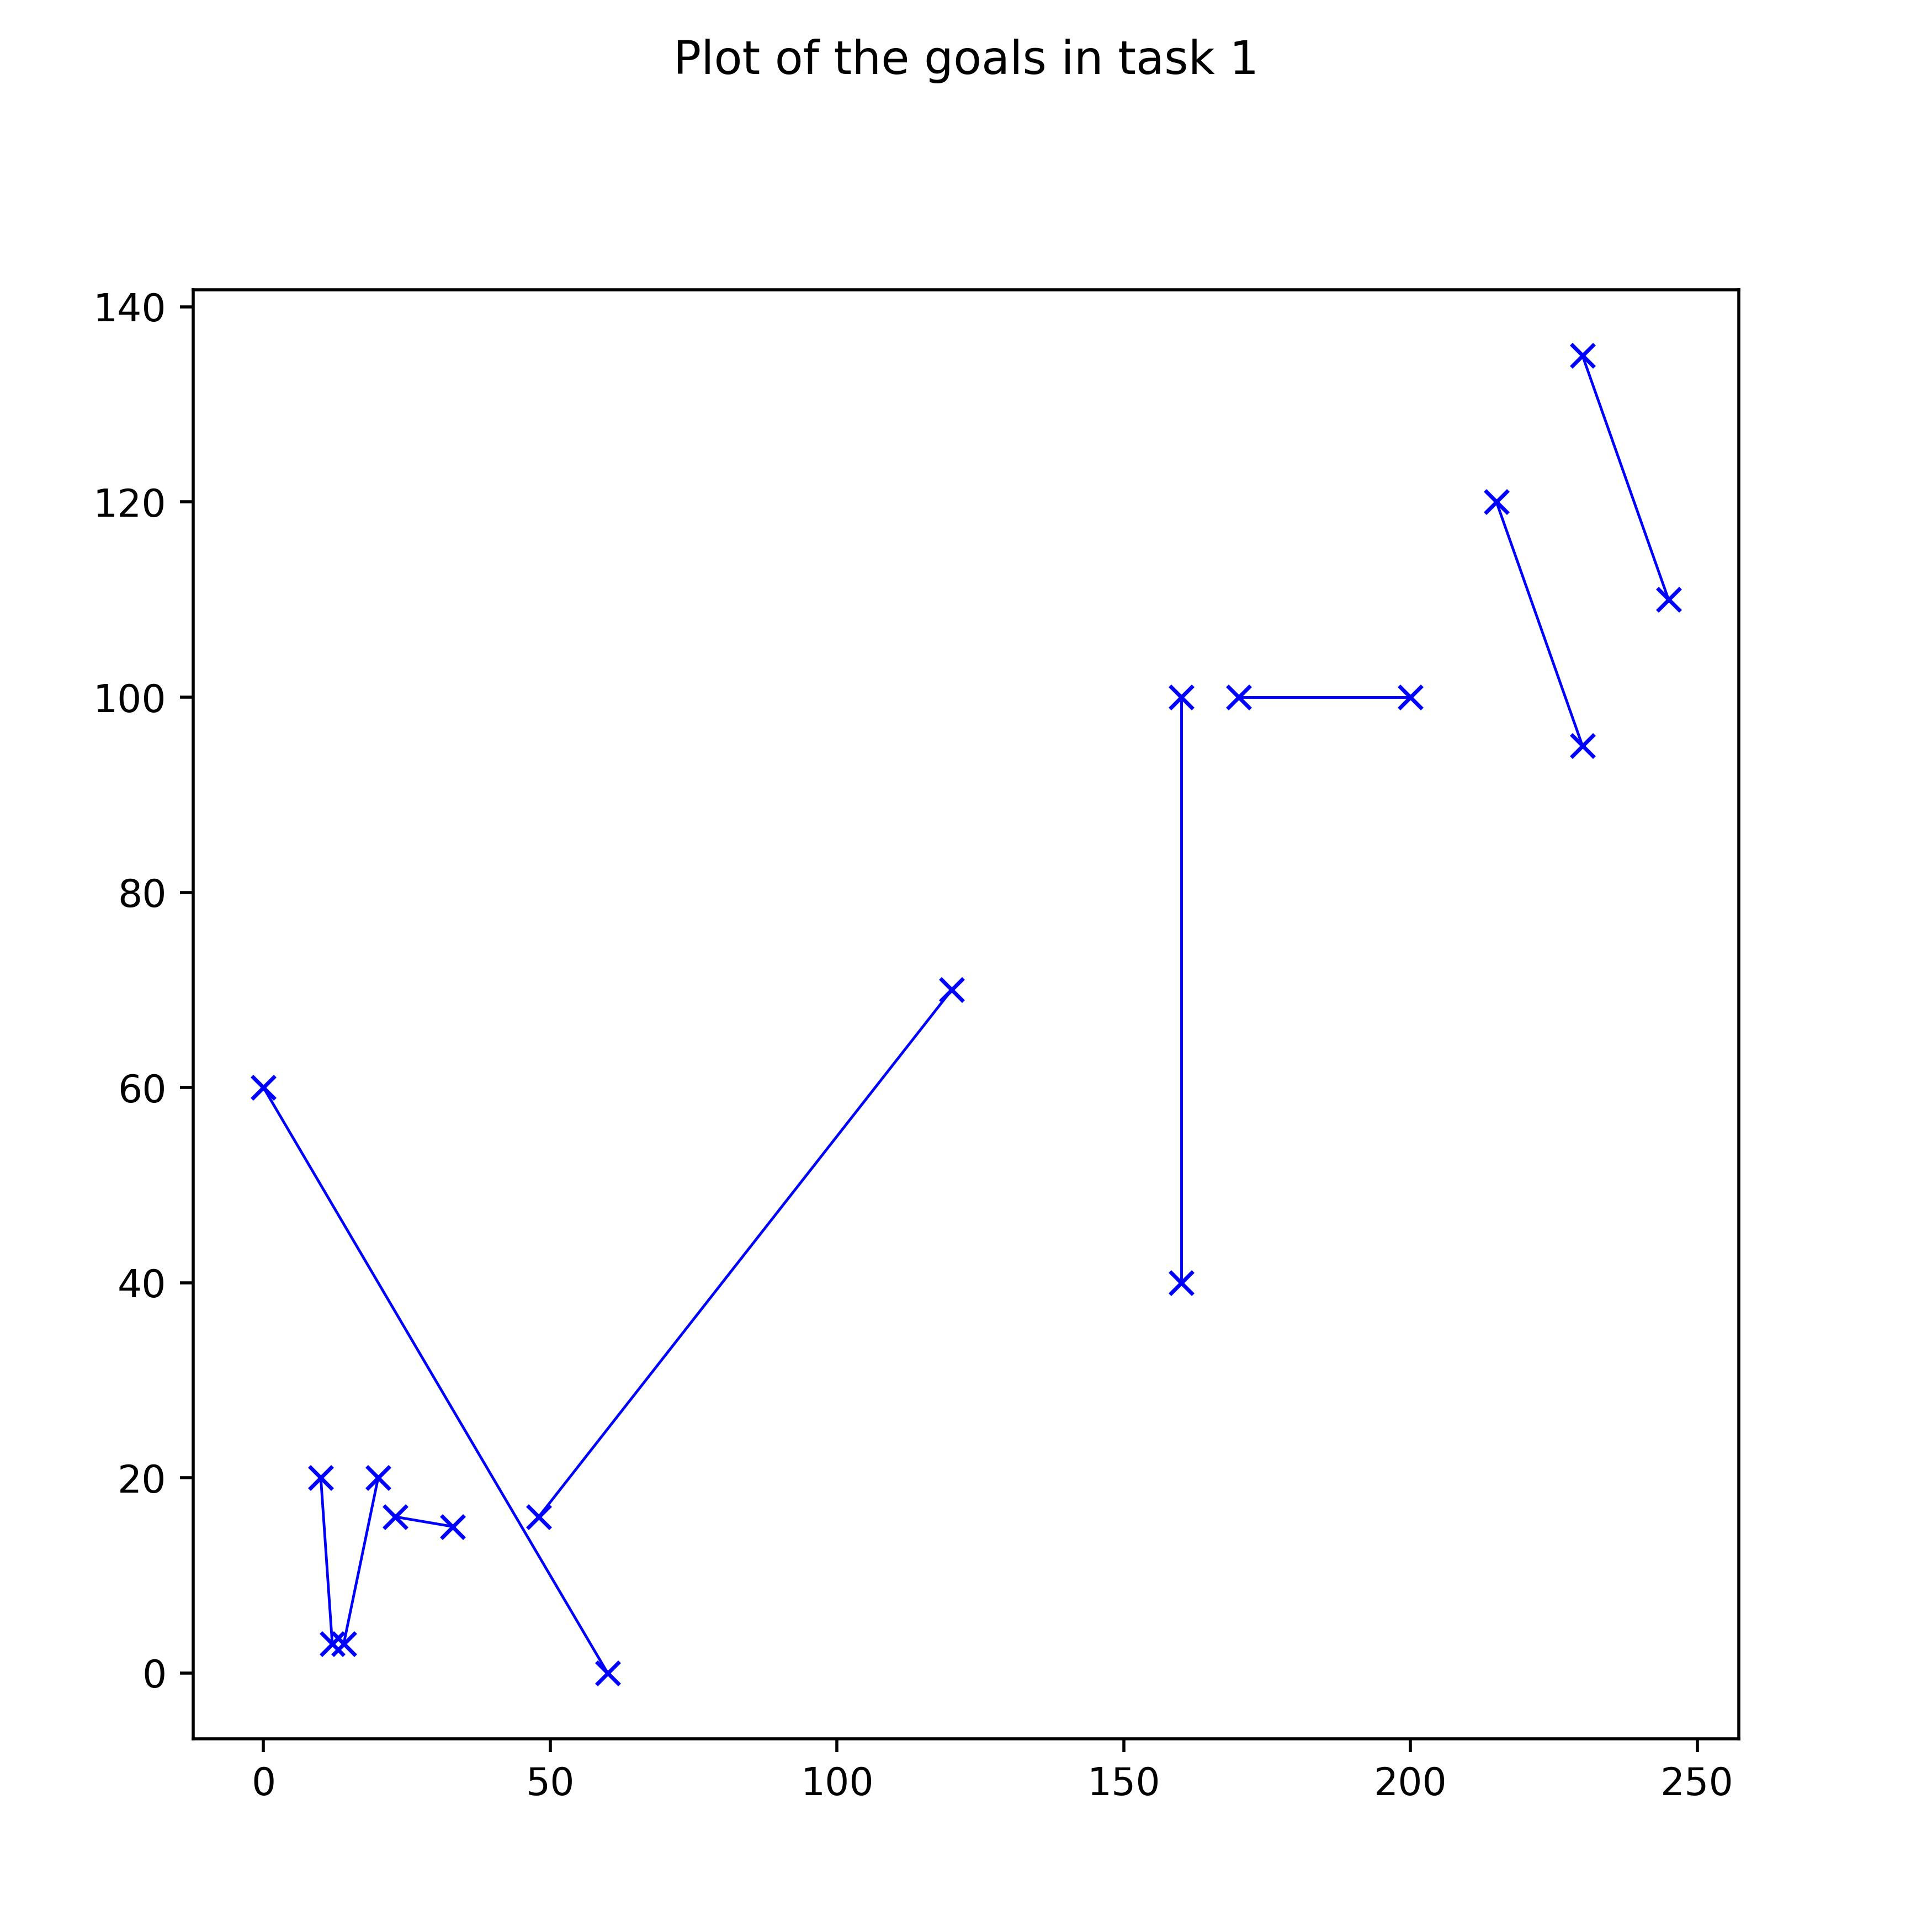
\includegraphics[width=\textwidth]{images/task_1.jpeg}
         \caption{Beispielaufgabe 1}
         \label{fig:y equals x}
     \end{subfigure}
     \hfill
     \begin{subfigure}[b]{0.49\textwidth}
         \centering
         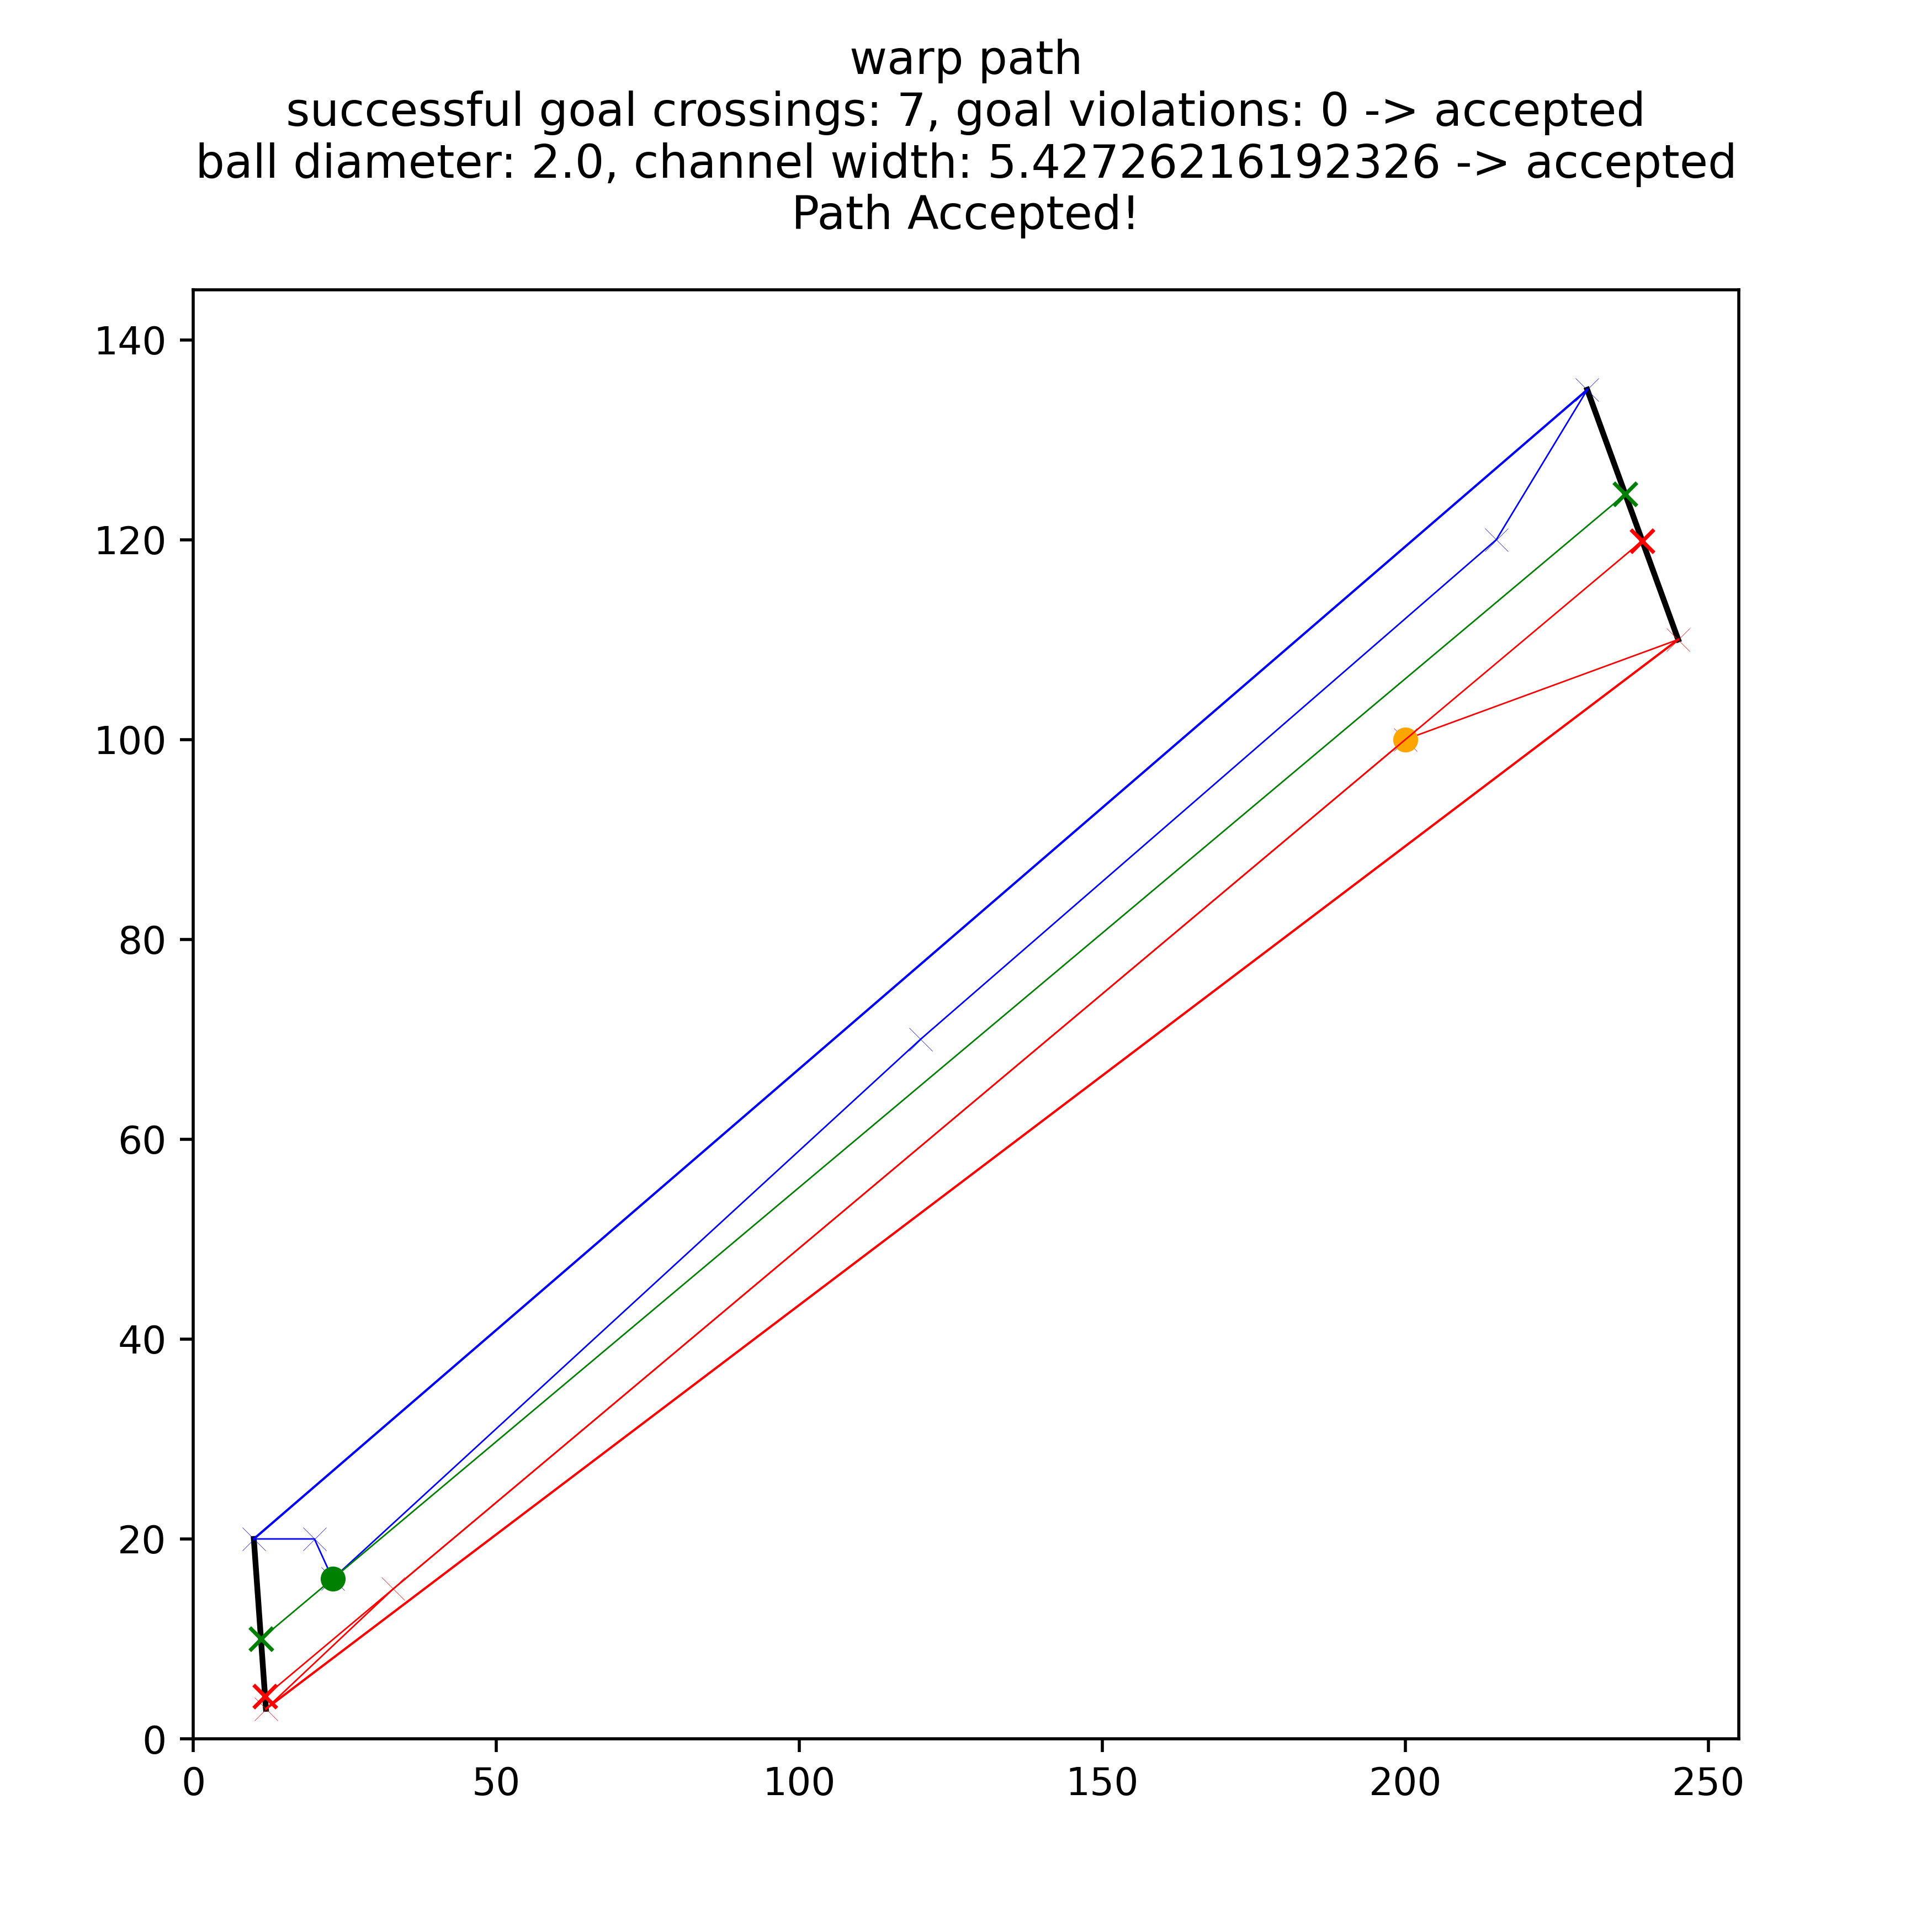
\includegraphics[width=\textwidth]{images/solution_task_1.png}
         \caption{Lösung der Beispielaufgabe 1}
         \label{fig:three sin x}
     \end{subfigure}
     \caption{Plot der Beispielaufgabe 1 und ihrer Lösung.}
        \label{fig:three graphs}
\end{figure}

\begin{figure}
\label{fig:beispiele2}
\vspace{-0.5cm}
\centering
     \begin{subfigure}[b]{0.49\textwidth}
         \centering
         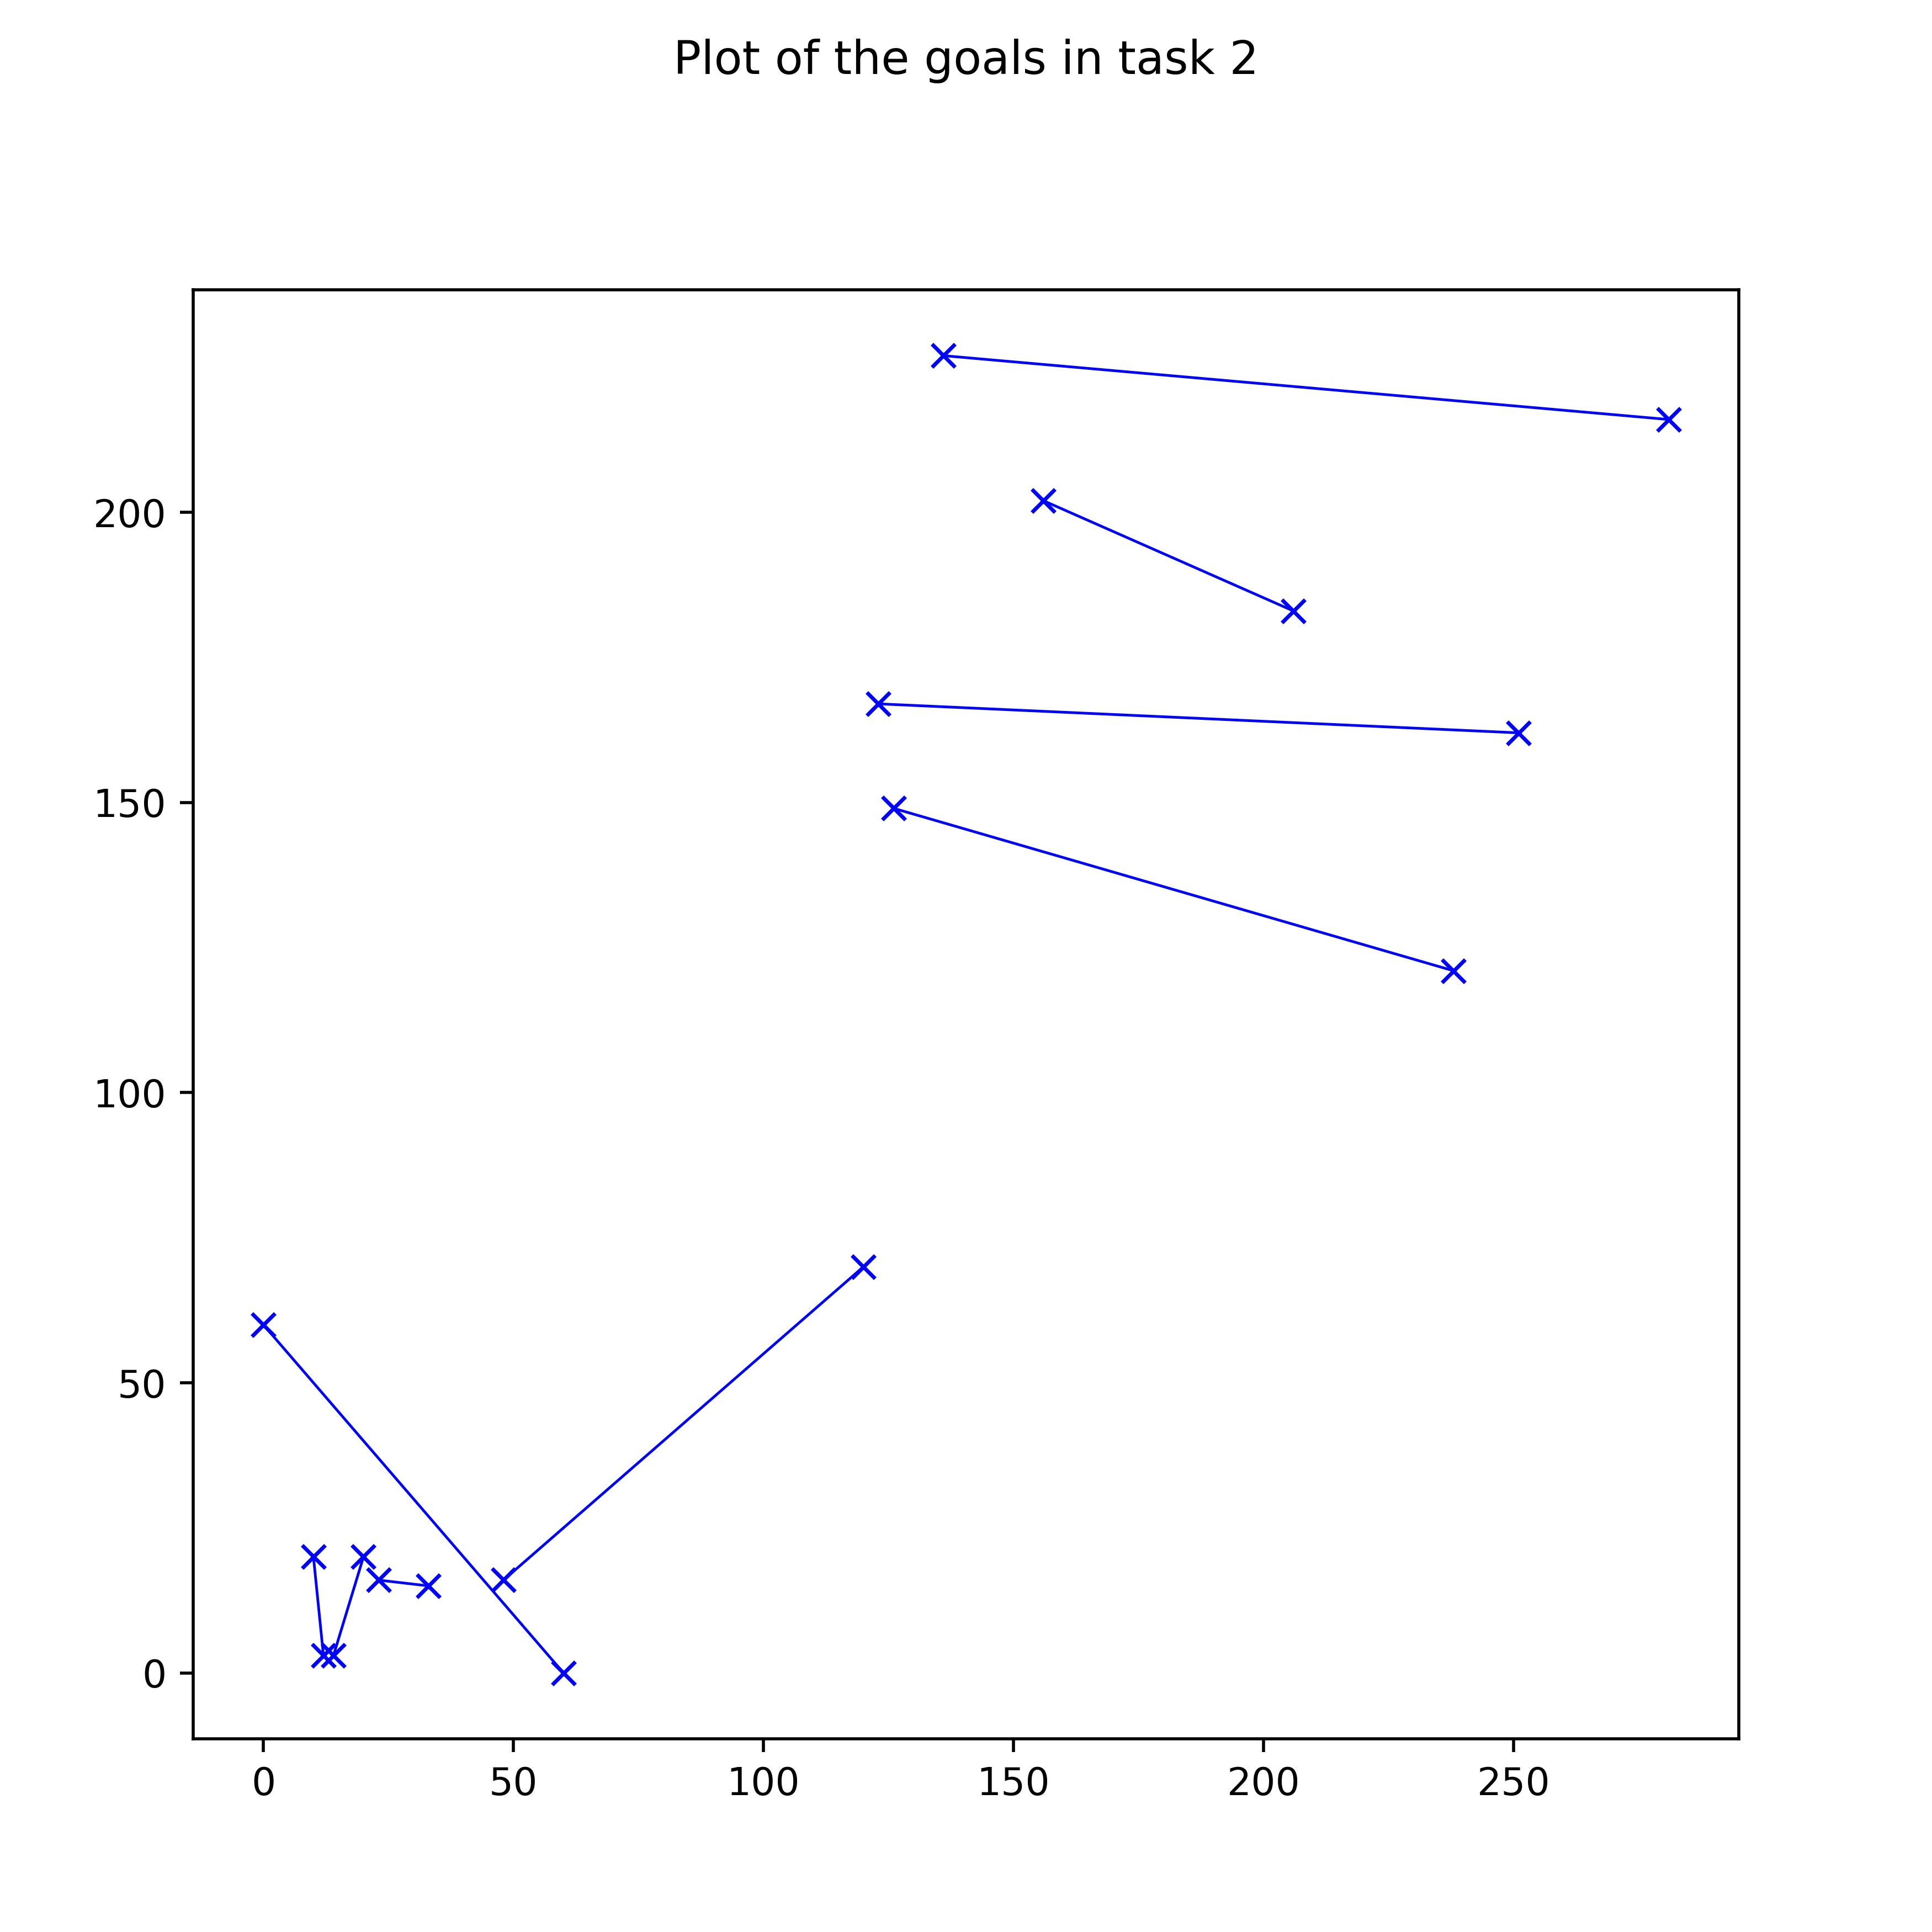
\includegraphics[width=\textwidth]{images/task_2.jpeg}
         \caption{Beispielaufgabe 2 besitzt keine Lösung, da es nicht möglich ist durch alle Tore zu schießen.}
         \label{fig:five over x}
     \end{subfigure}
     \hfill
     \begin{subfigure}[b]{0.49\textwidth}
         \centering
         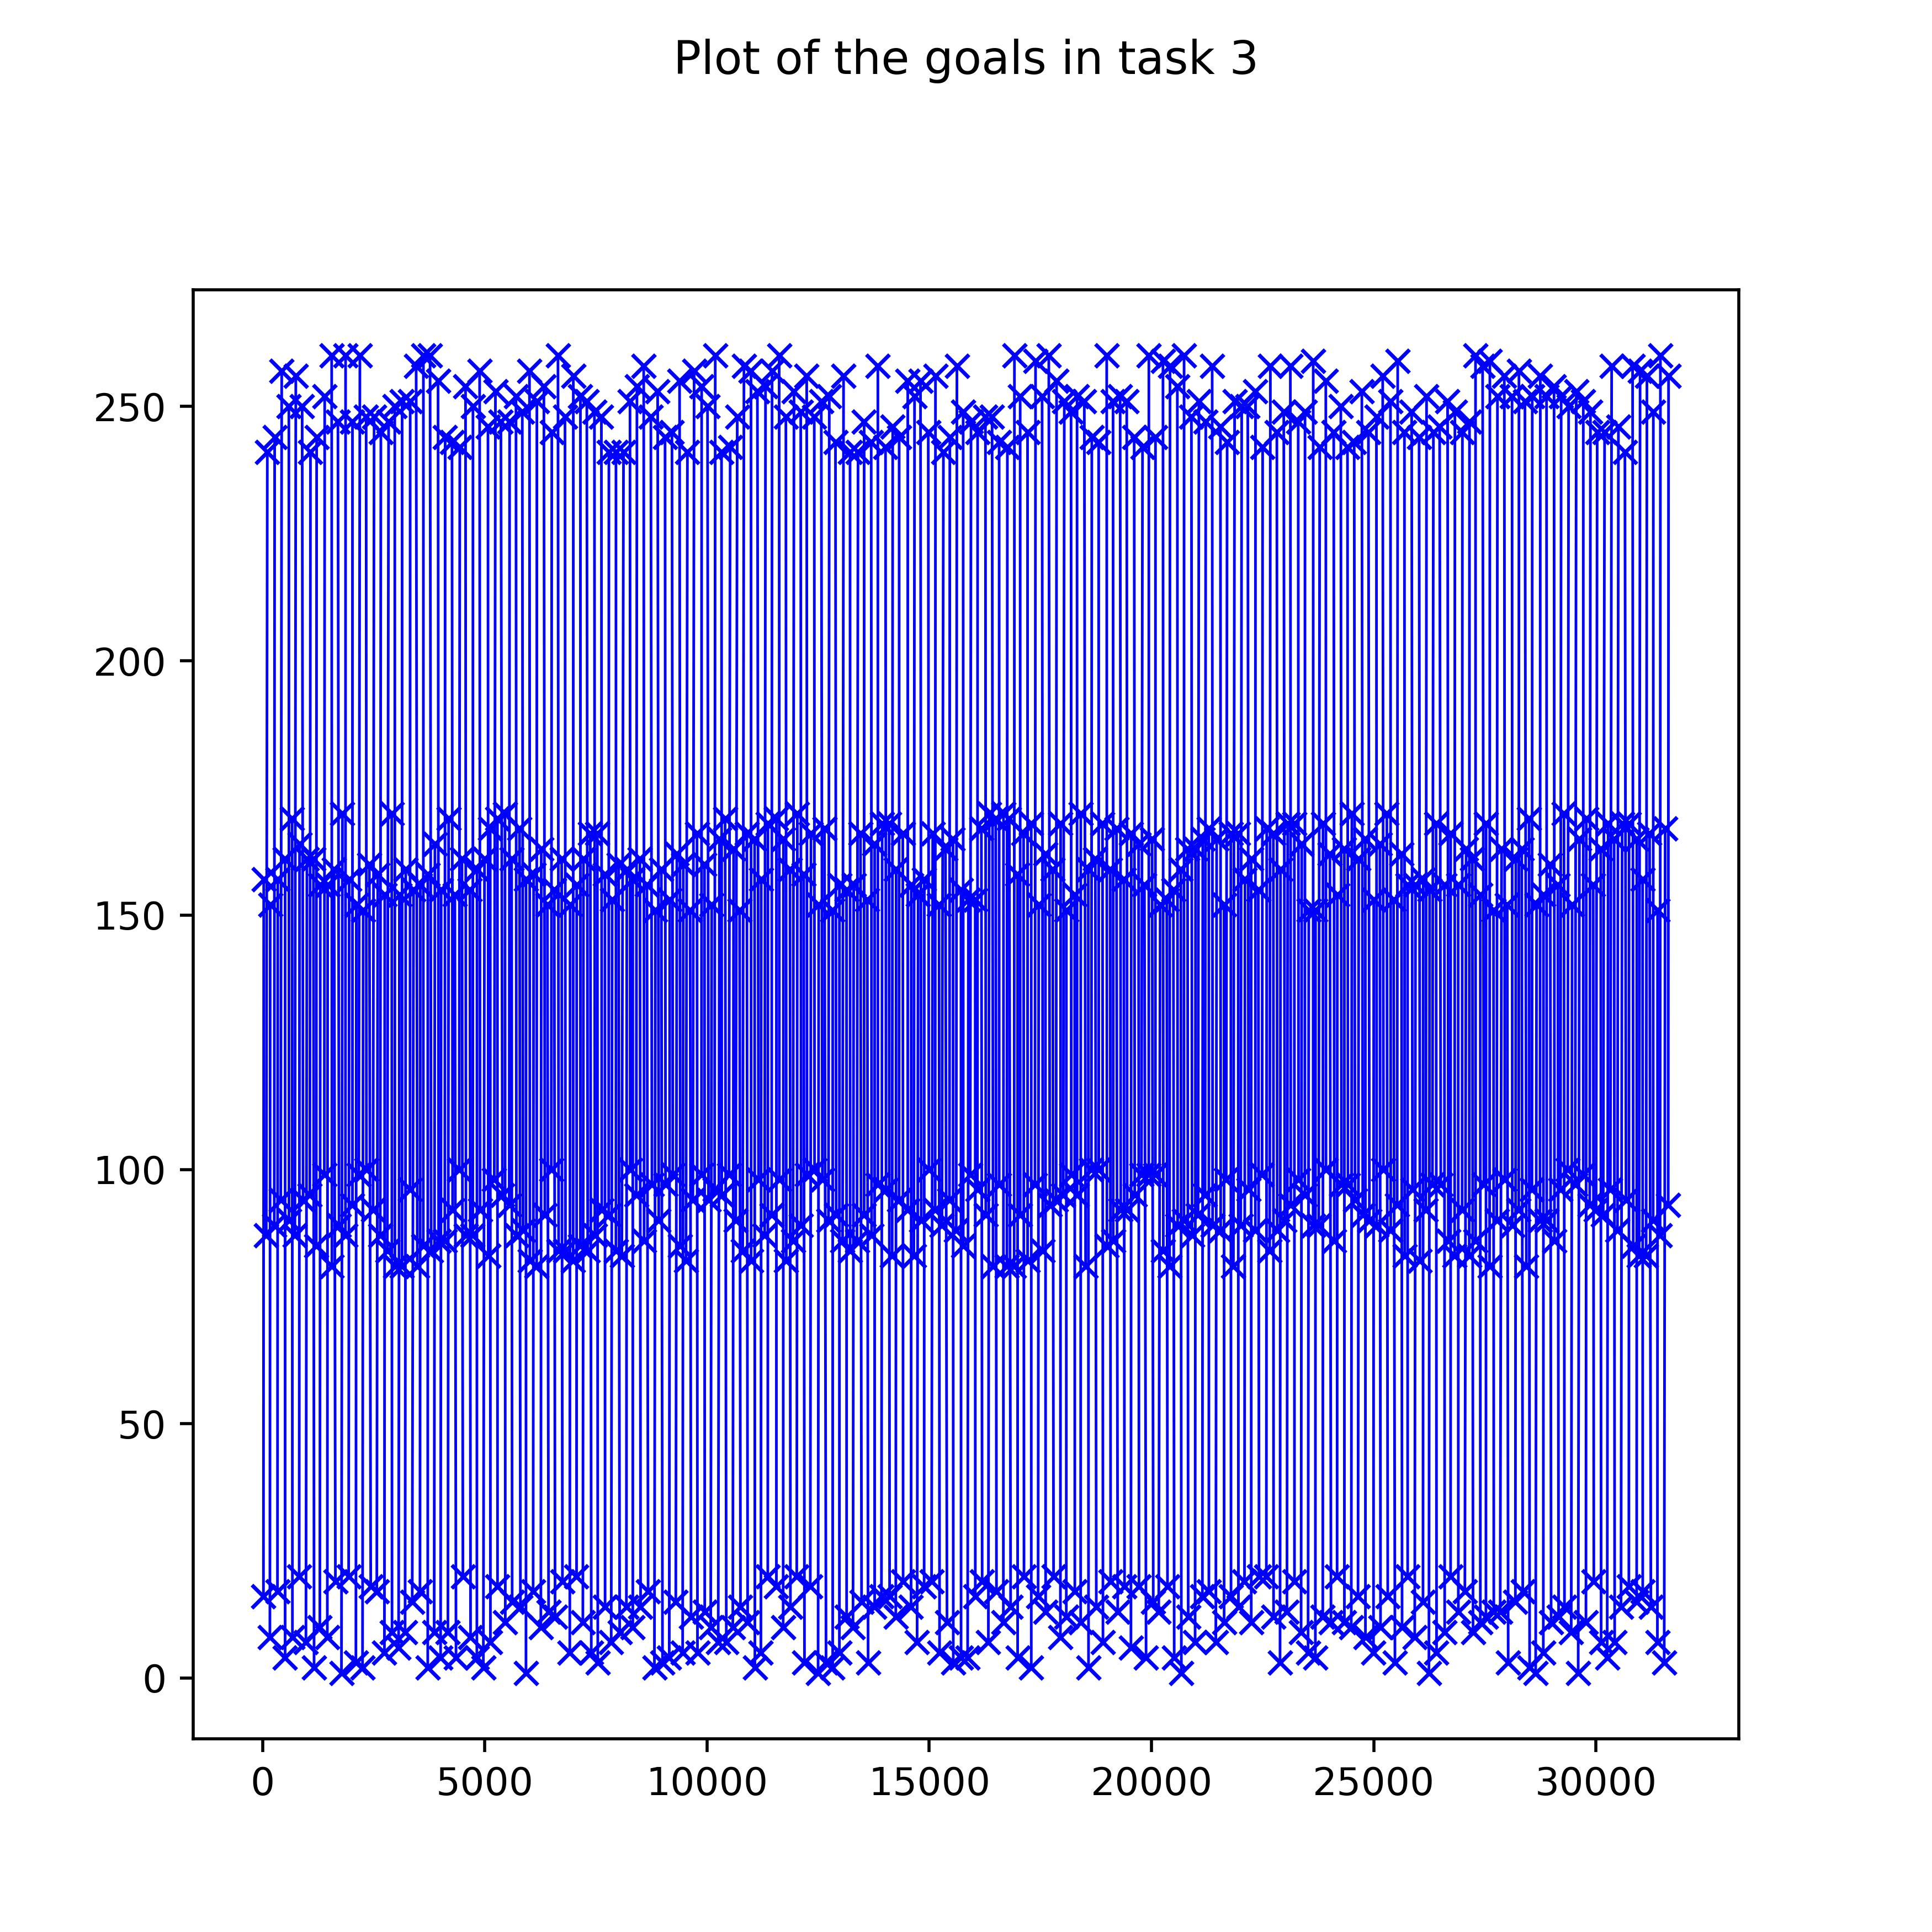
\includegraphics[width=\textwidth]{images/task_3.jpeg}
         \caption{Beispielaufgabe 3 besitzt keine Lösung, da die Tore in der falschen Reihenfolge sind.}
         \label{fig:five over x}
     \end{subfigure}
     \hfill
     \begin{subfigure}[b]{0.49\textwidth}
         \centering
         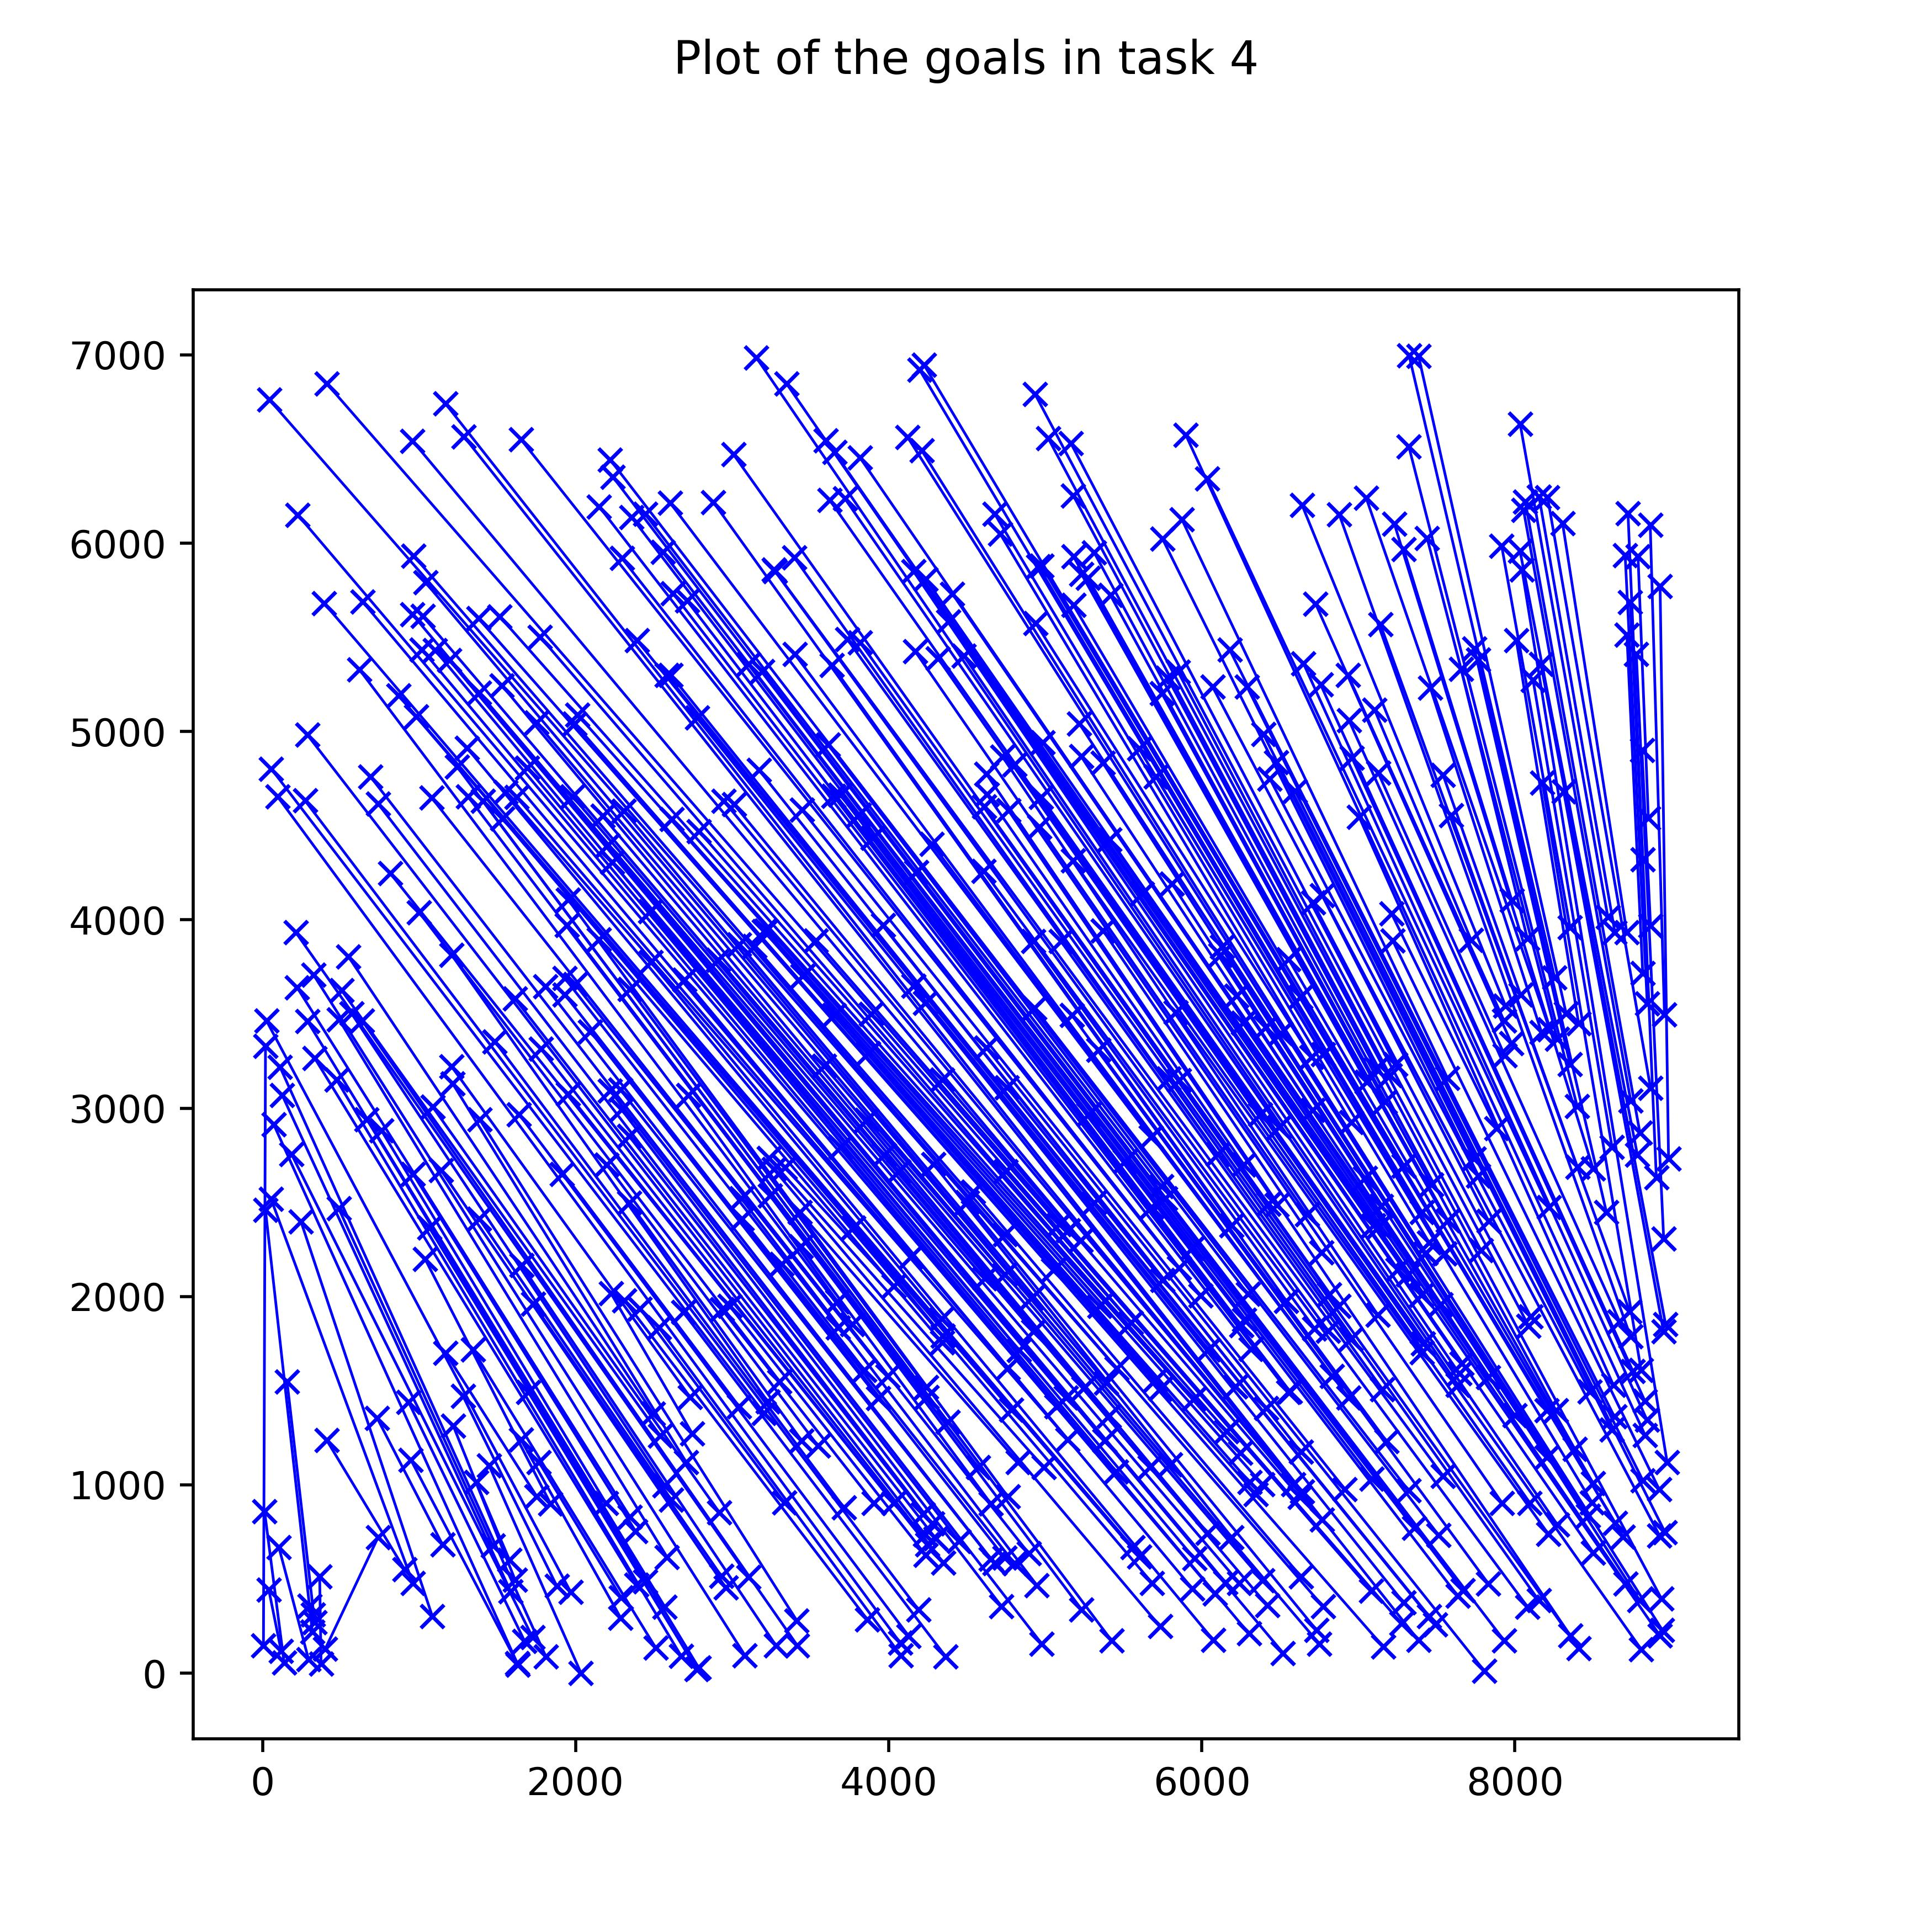
\includegraphics[width=\textwidth]{images/task_4.jpeg}
         \caption{Beispielaufgabe 4}
         \label{fig:five over x}
     \end{subfigure}
     \hfill
     \begin{subfigure}[b]{0.49\textwidth}
         \centering
         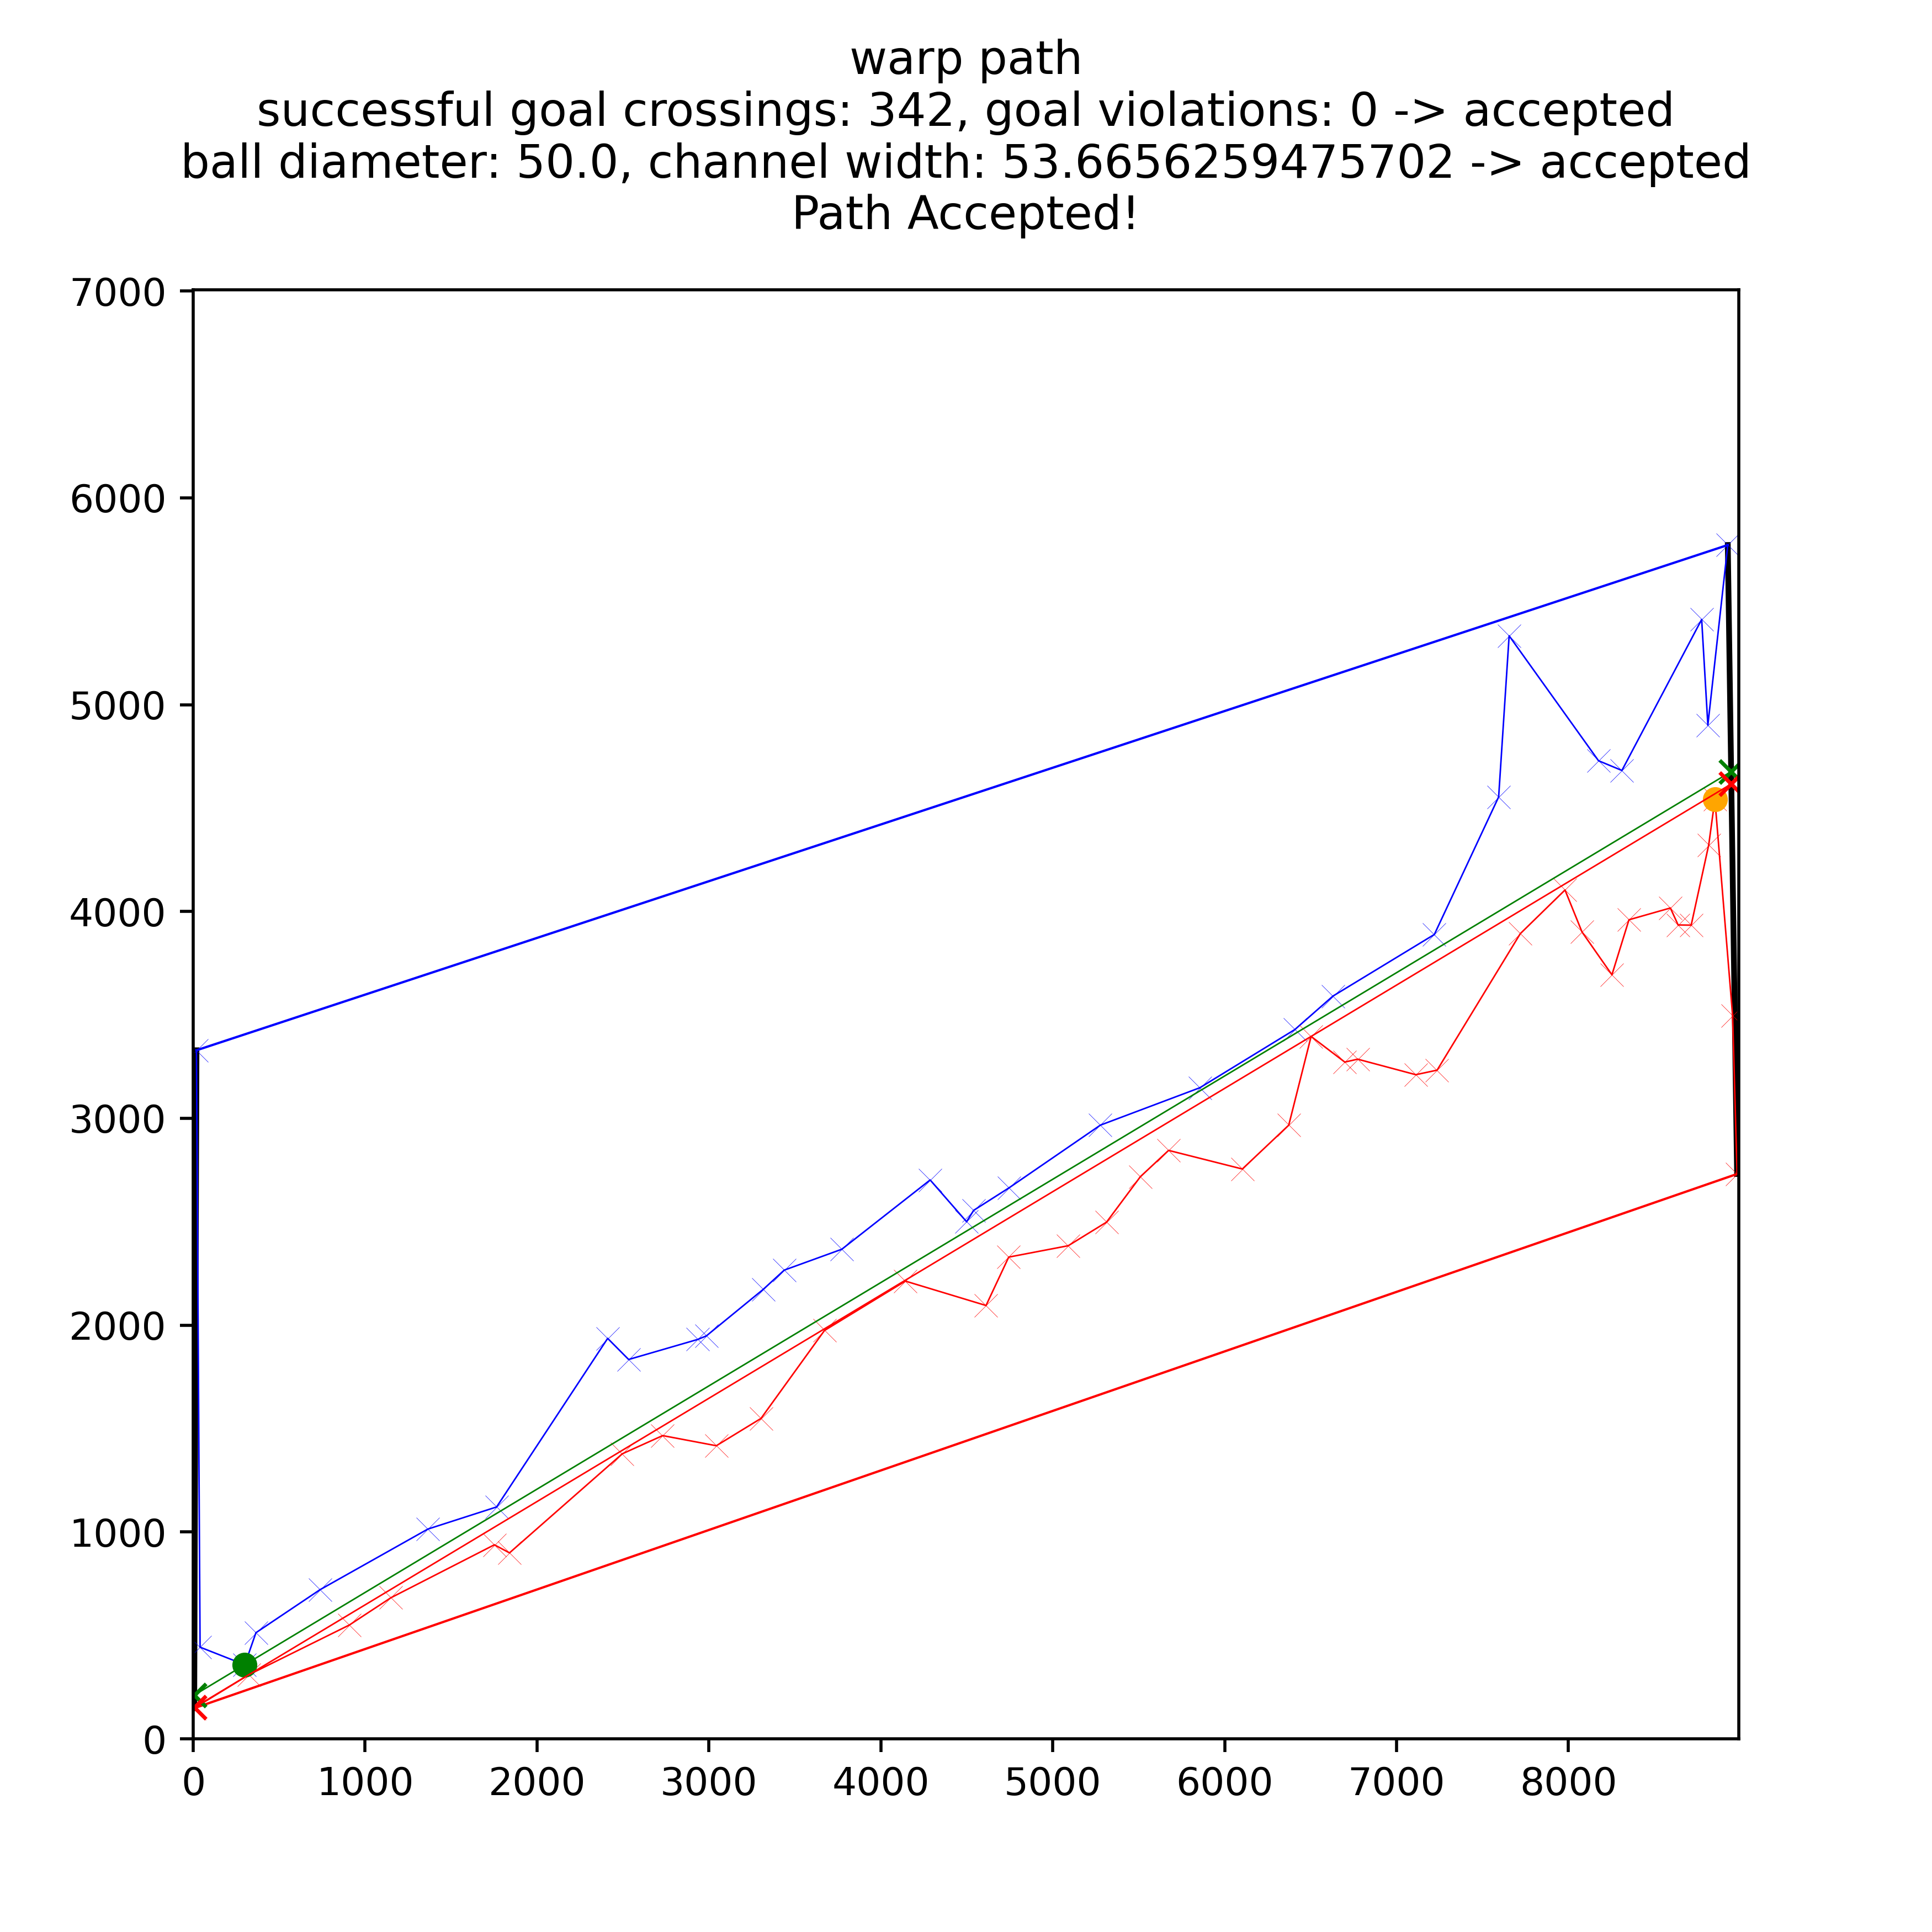
\includegraphics[width=\textwidth]{images/solution_task_4.png}
         \caption{Lösung der Beispielaufgabe 4}
         \label{fig:five over x}
     \end{subfigure}
          \hfill
     \begin{subfigure}[b]{0.49\textwidth}
         \centering
         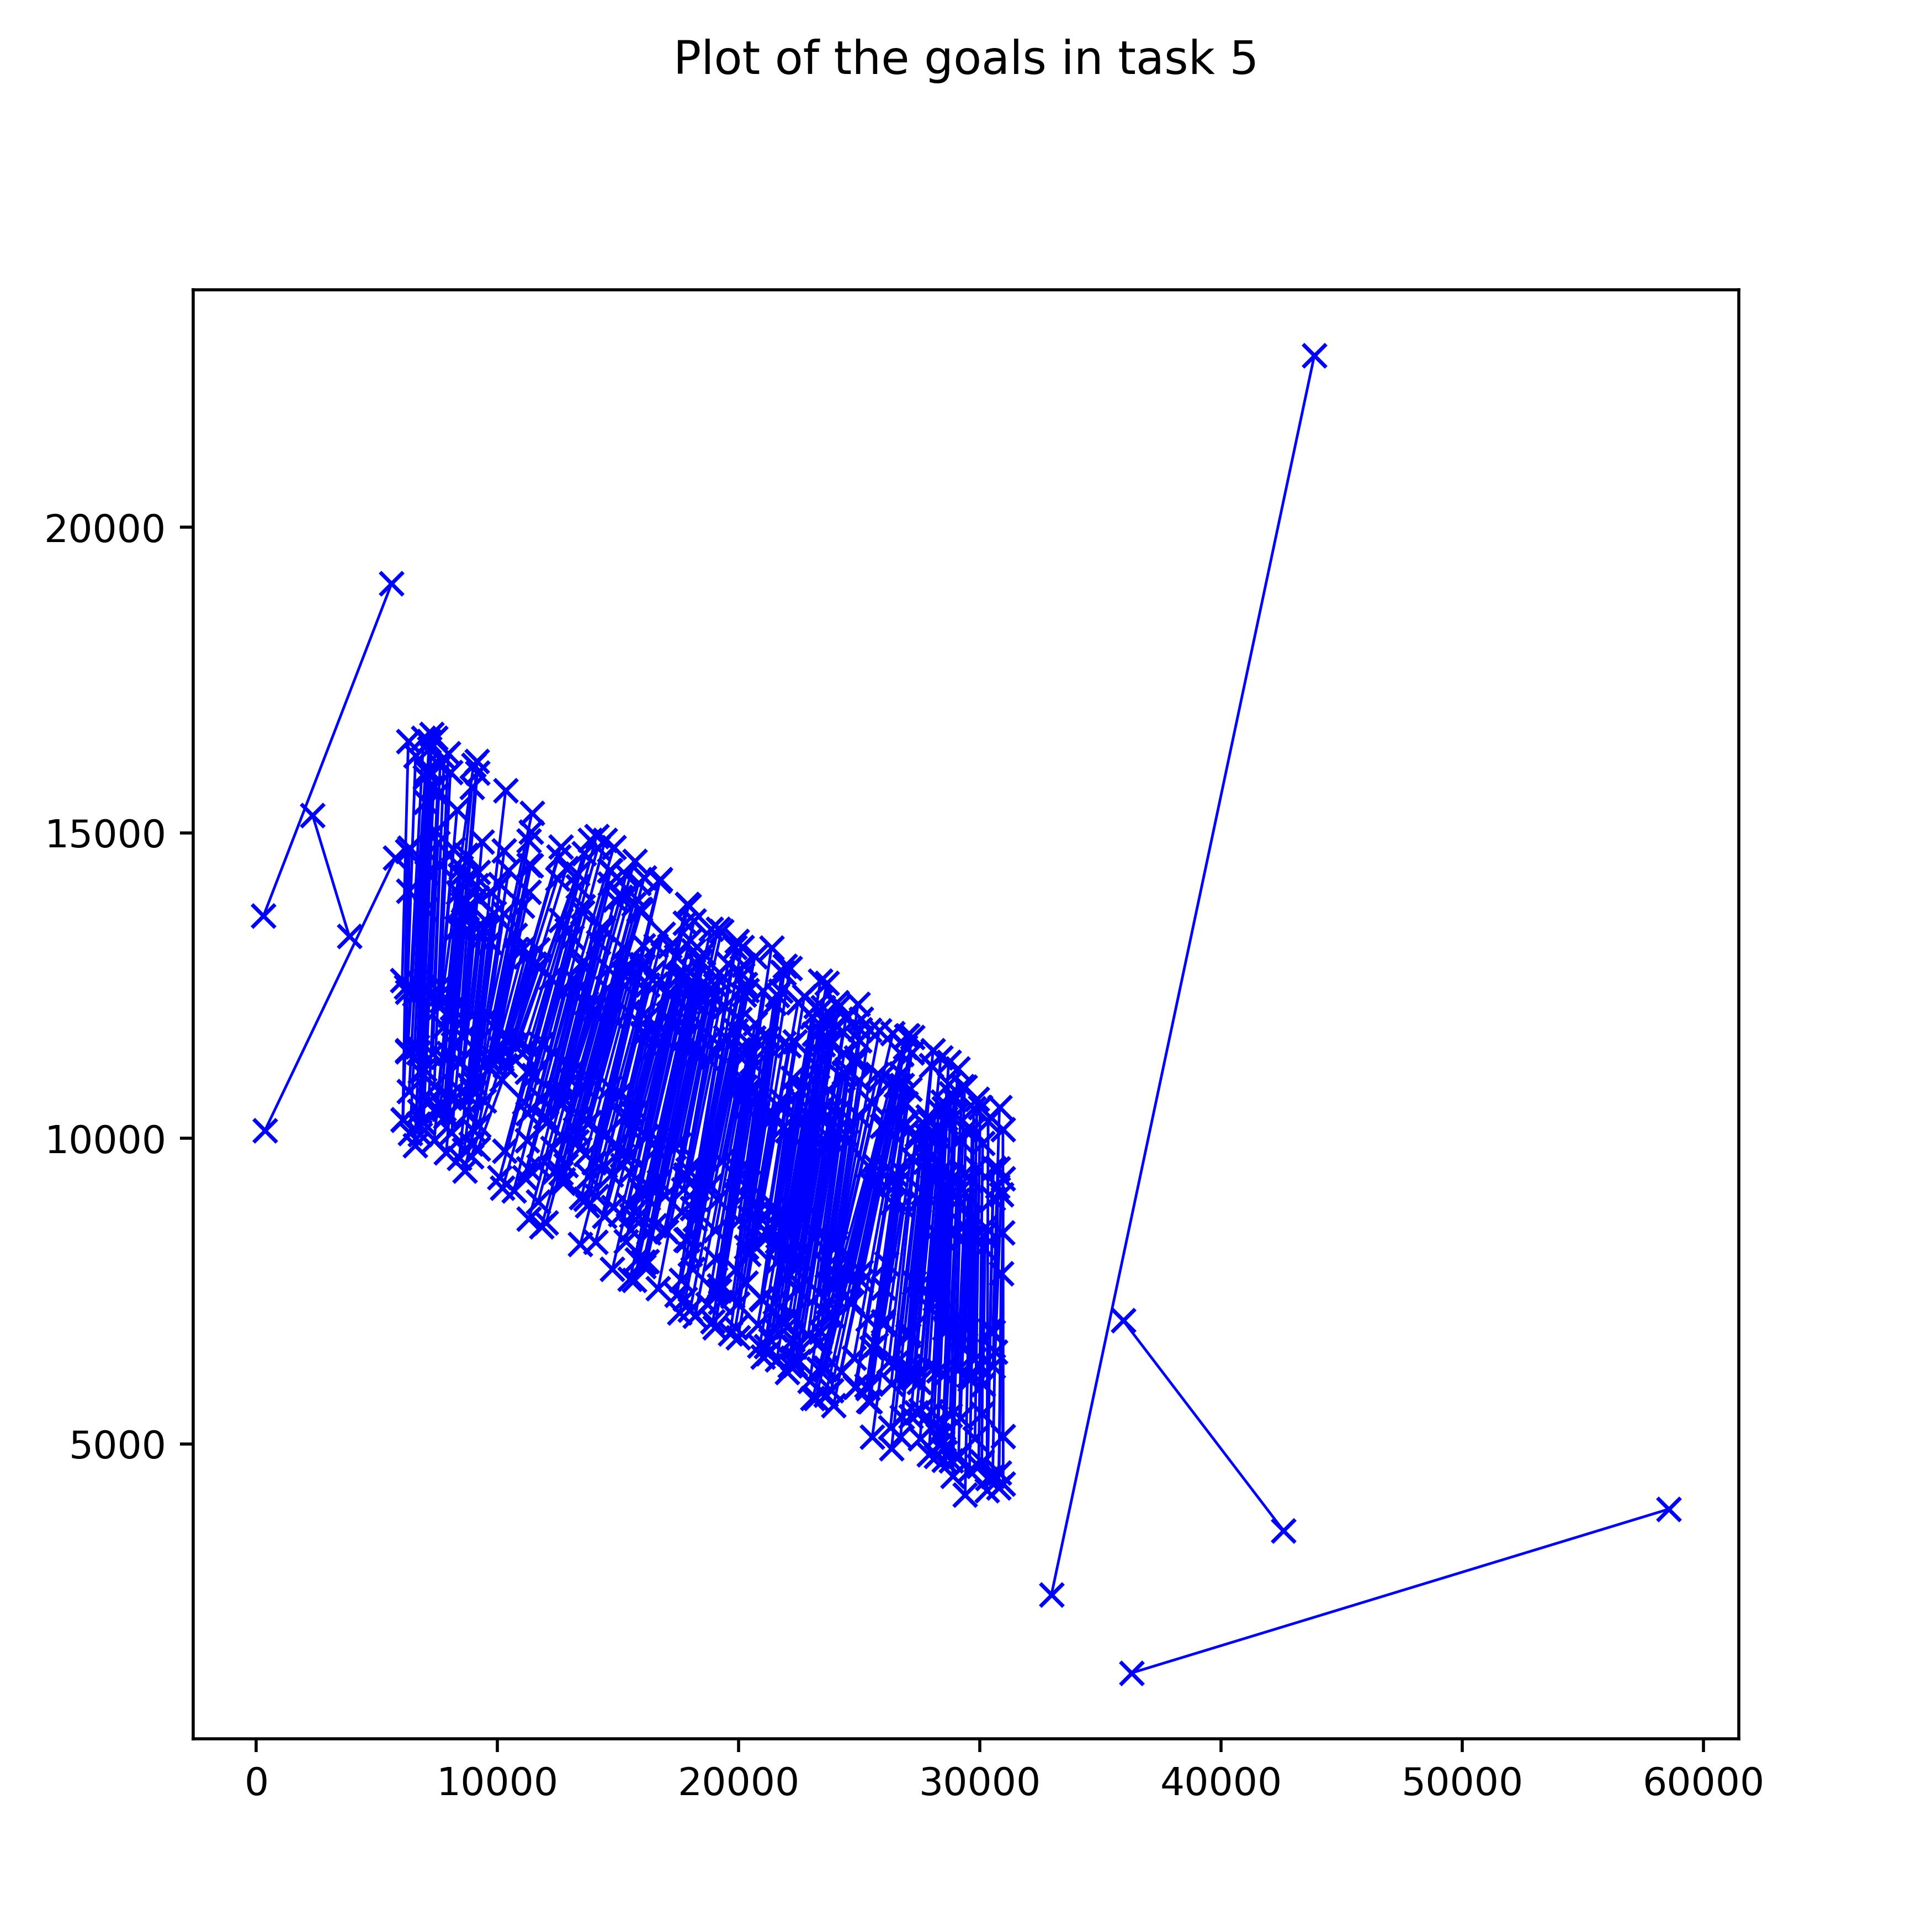
\includegraphics[width=\textwidth]{images/task_5.jpeg}
         \caption{Beispielaufgabe 5}
         \label{fig:five over x}
     \end{subfigure}
     \hfill
     \begin{subfigure}[b]{0.49\textwidth}
         \centering
         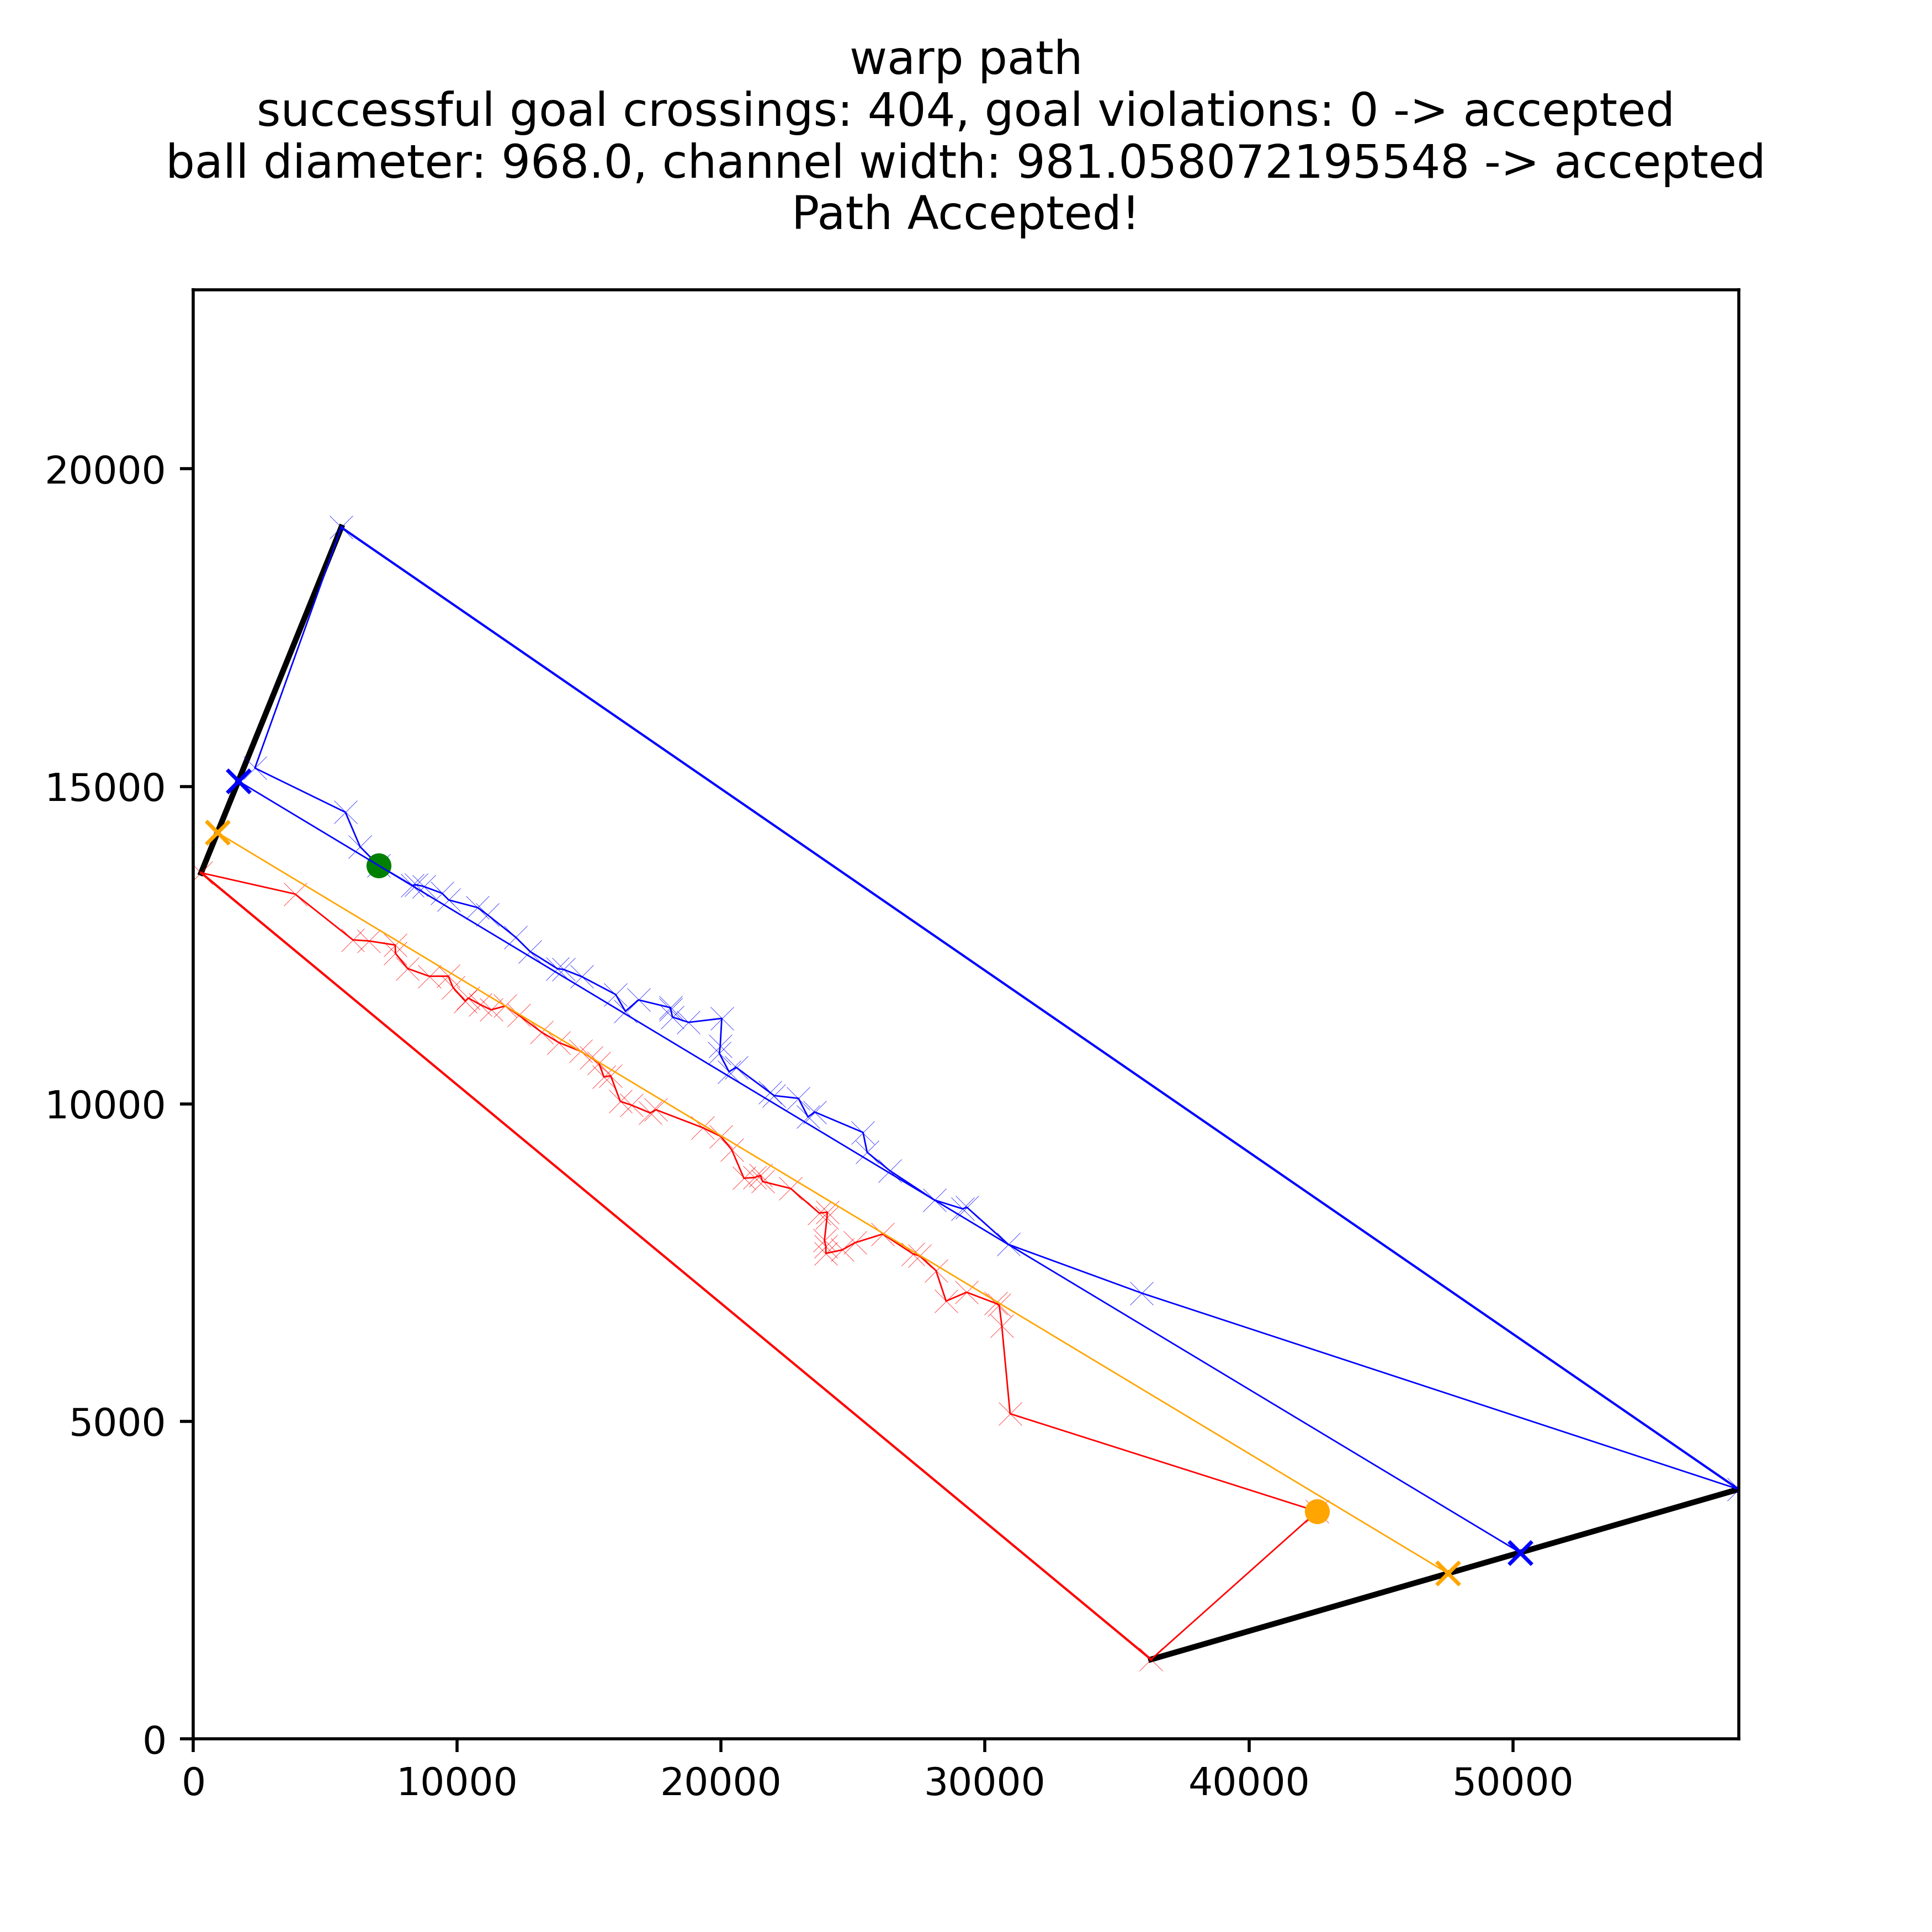
\includegraphics[width=\textwidth]{images/solution_task_5.png}
         \caption{Lösung der Beispielaufgabe 5}
         \label{fig:five over x}
     \end{subfigure}
        \caption{Plots der Beispielaufgaben 2 bis 5 und ihrer Lösung, sofern eine Lösung existert.}
        \label{fig:three graphs}
\end{figure}



\section{Schluss}

In der vorliegenden Komplexen Leistung wurde die Lösung der Krocket-Aufgabe detailliert analysiert und optimiert. Die zentrale Herausforderung bestand darin, einen effizienten, linearen Algorithmus zu entwickeln, der überprüft, ob ein Ball in der vorgegebenen Reihenfolge mit einem einzigen Schuss durch alle Tore geschossen werden kann. Durch den Einsatz von Konzepten wie Winkeltests, Isoklinen und verzerrten Ebenen konnte die Laufzeitkomplexität erheblich verbessert werden. Der entwickelte Ansatz stellt somit eine bedeutende Verbesserung gegenüber dem ursprünglichen Brute-Force-Algorithmus dar.

Die Zielsetzung der Arbeit wurde erreicht: Es wurde ein Algorithmus entwickelt, der es ermöglicht, für beliebige Konfigurationen von Toren eine Lösung effizient zu berechnen oder nachzuweisen, dass keine Lösung existiert.

Mir hat die Erarbeitung der Komplexen Leistung gezeigt, wie bedeutend eine systematische Herangehensweise an komplexe Fragestellungen ist. Durch die Fehleranalyse und kontinuierliche Optimierung wurde mir immer wieder verdeutlicht, wie essenziell eine präzise und strukturierte Denkweise in der Informatik ist. Die eigenständige Einarbeitung hat meine persönliche Kompetenz in diesen Bereichen erheblich gesteigert.

Die Erkenntnisse dieser Arbeit besitzen nicht nur theoretische Relevanz, sondern lassen sich auch in praktischen Anwendungen der Robotik nutzen. Ein konkretes Beispiel hierfür ist die Laufpfaderkennung autonomer Roboter, die – ähnlich wie in der Krocket-Aufgabe – Hindernisse in einer bestimmten Reihenfolge passieren müssen. Die Konzepte der Chokepoints und Isoklinen lassen sich auf die Bewegungsplanung und Navigation dieser Roboter übertragen. Das Team der HTWK-Robots, dem ich angehöre, prüft derzeit mögliche Integrationen des Algorithmus in der Laufpfaderkennung sowie in der Schussplanung, da die Roboter zunächst feststellen müssen, ob ein Schusspfad nicht durch Hindernisse blockiert ist.

Eine mögliche Erweiterung des Algorithmus, die die Option eines doppelten Schusses berücksichtigt, wäre sinnvoll. So wäre die Planung von Passspielen oder komplexeren Manövern denkbar. Dies würde neue Herausforderungen hinsichtlich der optimalen Schussaufteilung und strategischen Positionierung mit sich bringen. Auch eine Berechnung der Schusskraft wäre hilfreich, um zu bestimmen, ob der Schuss physisch überhaupt realisierbar ist.

\textbf{Zusammenfassend} bietet diese Arbeit eine algorithmische Lösung für eine anspruchsvolle Problemstellung. Der entwickelte Algorithmus besitzt vielfältige Anwendungsmöglichkeiten, beispielsweise in der Laufpfadberechnung, und bietet Potenzial für zukünftige Weiterentwicklungen. Die vorliegende Komplexe Leistung zeigt darüber hinaus, wie augenscheinlich einfache Probleme keineswegs einfache Lösungen haben müssen, da diese entweder sehr rechenintensiv wie der Brute Force Algorithmus sind oder erheblicheren konzeptuellen Aufwand erfordern.

\printbibliography[heading=bibnumbered]
\newpage
\thispagestyle{empty}
\section{Selbstständigkeitserklärung}
Hiermit bestätige ich, dass ich die vorliegende Arbeit eigenständig (ohne KI) verfasst und
keine anderen als die angegebenen Hilfsmittel und Quellen verwendet habe.
Alle wörtlich oder sinngemäß übernommenen Stellen im Text anderer Quellen wurden
kenntlich gemacht.\\

Leipzig, den 13. Februar 2025



\end{document}
